\chapter{图上的组合优化}
\label{chap:graph-optimization}

前两章研究图上“有什么连接”和“怎样把连接找出来”：第~\ref{chap:graph-objects}章定义路径、树与分隔，第~\ref{chap:graph-traversal}章用遍历恢复路径、提取连通结构、排出依赖次序。那里的问题大多只问存在与否，一条路线或一棵生成树只要满足结构要求就算完成。本章给边配上数值，并在满足结构要求的众多候选中挑出数值最好的一个。在同一张交通网络上，可以选一条总长度最短的路线，可以铺一组总造价最低、又能连通所有站点的线路，也可以在每条道路的通行上限内安排尽可能多的输送量。三个问题的选择对象分别是一条路径、一组边和每条弧上的一个数，边旁的数字分别表示长度、造价和容量。因此，每个问题都要先固定选择对象与目标，再讨论算法。

本章依次处理六个问题。第~\ref{sec:graph-shortest-paths}节在有向图上寻找起点到各顶点的最短路。三种算法共用“距离标签”和“松弛”两个操作：有向无环图按拓扑序一遍完成；Bellman--Ford算法允许标签反复修正，并能识别负环的影响；Dijkstra算法在边长非负时每次永久确定一个顶点。第~\ref{sec:graph-minimum-spanning-tree}节在无向图上选总权最小的生成树，Kruskal算法与Prim算法都依靠同一条割性质，用交换论证说明每次选边是安全的。第~\ref{sec:graph-max-flow}节在容量限制下最大化源到汇的输送量，引入可以撤回旧流量的残量网络。它证明一个可行流最优当且仅当残量网络中没有增广路径，并由按最少弧数选路的Edmonds--Karp算法得到“最大流值等于最小割容量”。

后三节在最大流的基础上改变目标或结构。第~\ref{sec:graph-min-cost-flow}节固定各点的供需量，转而最小化输送费用。最优性改由残量网络中没有负费用环来刻画，网络单纯形法把可行流组织成生成树，沿树上的基本环逐步降低费用。第~\ref{sec:graph-matching}节在二部图中选取互不共享端点的边，交替路径扮演增广路径的角色，单位容量的流网络把匹配和最大流联系起来。第~\ref{sec:graph-assignment}节要求每个对象都完成配对并最小化总成本，匈牙利算法同时维护给出成本下界的顶点标号与由紧边组成的匹配，两者相遇时即得最优解。

六个问题的算法各不相同，论证却有共同的样式：先指出算法维护什么状态，再说明哪一条递推、交换或上下界论证排除了更好的候选，最后交代计算开销与条件失效时会发生什么。许多算法除了给出答案，还附带一份可以独立复核的“证书”，如最短路的逐弧不等式、同值的流与割、同值的指派与标号。第~\ref{sec:graph-optimization-summary}节把这些证书与各自的成立条件并列比较。全章记顶点数为$n=|V|$，无向边数为$m$，有向弧数为$a$。除非另有说明，图以邻接表存储，边长、容量、成本等数值另存在与边对应的数组中。

% 第3章第1节：最短路（路径成本与三类距离结果、距离标签与松弛、DAG递推、Bellman--Ford、Dijkstra、方法比较与结果检验）。

\section{最短路}
\label{sec:graph-shortest-paths}

第~\ref{sec:graph-bfs}节的广度优先遍历给出从起点出发的最少边数。可是在道路网络中，每段路的长度不同；在任务调度中，从一个状态转到另一个状态的代价也各不相同。这时要比较的是路线上各段数值之和，经过的边数少不等于总成本低。

本节在有向加权图上研究这个问题。先说明路线成本怎样定义、距离可能出现哪几类结果，再建立三种算法共用的距离标签与松弛操作。随后依次介绍三种算法：有向无环图上的递推利用无环次序，Bellman--Ford算法允许标签反复修正，Dijkstra算法在边长非负时永久确定标签。每种算法的正确性论证紧接在各自的机制之后，最后比较三者的适用范围，并说明怎样检验一份最短路结果。

\subsection{路径成本与最短路问题}
\label{sec:graph-opt-path-cost}

设$\mathcal G=(V,E)$是有限有向图，每条弧$u\to v$带有一个实数\emph{长度}$\ell_{u,v}$。长度可以表示距离、时间或转换代价，也允许为负，例如某次转换带来收益。对一条行走$W=(v_0,v_1,\ldots,v_k)$，规定它的成本为沿途弧长之和：
\[
  \ell(W)=\sum_{r=1}^{k}\ell_{v_{r-1},v_r}.
\]
只含一个顶点的零步行走成本为零。所有长度都等于$1$时，成本就是边数，回到广度优先遍历的情形；一般长度下两者不再一致。例如$s$到$t$有一条长$5$的直达弧，又有经过$u$、两段各长$1$的路线，两步路线反而更短。

\paragraph{两种候选集合}
寻找“最短路线”时，必须先说清候选集合是什么。一种选择只允许简单路径，即不重复经过顶点的路径；另一种允许一般的行走，顶点和弧都可以重复。有限图中简单路径只有有限条，因此只要终点可达，最小值一定存在；行走可以无限地绕圈，候选有无穷多个，只能谈成本的下确界。

\begin{definition}[最短路问题]
\label{def:graph-opt-shortest-path}
给定有限有向图$\mathcal G=(V,E)$、弧长$\ell_{u,v}\in\mathbb R$与源点$s\in V$。对每个顶点$v$，记$\mathcal W_{s,v}$为从$s$到$v$的全部有限行走组成的集合，称
\[
  \delta(v)=\inf_{W\in\mathcal W_{s,v}}\ell(W)
\]
为$s$到$v$的\term{最短路}距离，约定空集的下确界为$+\infty$。若某条行走$W\in\mathcal W_{s,v}$满足$\ell(W)=\delta(v)$，就称$W$是一条$s$到$v$的最短路。求出全部$\delta(v)$及相应路线的问题称为单源最短路问题。
\end{definition}

本节的算法计算的都是行走下确界$\delta(v)$。在多数情形中它与简单路径的最小值一致，原因是行走中的绕圈部分可以删掉。设行走$W$两次经过顶点$x$，两次之间的一段是从$x$回到$x$的闭行走$C$，删去$C$得到更短的行走$W'$，并且$\ell(W')=\ell(W)-\ell(C)$。只要$C$的成本非负，删去它就不会增加成本。反复删除，直到不再有重复顶点，便得到一条成本不超过$\ell(W)$的简单路径。

\paragraph{负环与三类结果}
删除闭合段的论证只在闭行走成本非负时有效。成本为负的有向环称为\term{负环}（negative cycle）。若能从$s$走到某个负环，绕若干圈后再走到$v$，则每多绕一圈，成本就再降低一次，于是$\delta(v)=-\infty$。这并不表示存在一条“长度为负无穷的路径”，而是说任何有限成本都能被另一条行走打破。反过来，若没有这样“从$s$可达、又能到达$v$”的负环，那么$s$到$v$的行走中出现的任一闭合段也不可能为负。原因是一条成本为负的闭行走，在第一个重复顶点处切开，总能分出一个简单环，剩下的部分仍是闭行走；重复这一切分，闭行走的成本就写成若干个简单环的成本之和，其中必有一个为负，而这个环同样从$s$可达、又能到达$v$。因此在这种情形下，所有闭合段都可以删除，$\delta(v)$等于简单路径的最小成本，并且由一条简单路径达到。

综上，一次单源查询中，每个顶点的距离属于三类之一：不可达时$\delta(v)=+\infty$；可达且不受负环影响时$\delta(v)$为有限值，并由一条简单路径达到；能从某个$s$可达的负环到达时$\delta(v)=-\infty$。三类顶点可以出现在同一张图中。图~\ref{fig:graph-opt-distance-outcomes}中，负环$a\to b\to a$只影响它自己及其后继$t$；旁支$u$不能从这个负环到达，距离仍是有限的$4$；另一个负环$x\to y\to x$从$s$出发到不了，对本次查询没有任何影响。所以不能因为图中某处有负环，就把全部顶点都标成负无穷。

\begin{figure}[!htb]
  \centering
  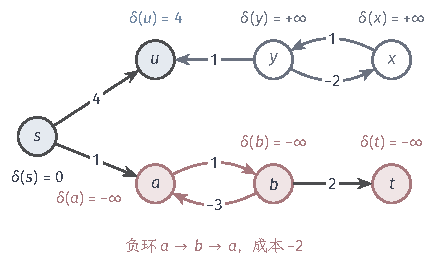
\includegraphics[width=73.801mm]{figures/01-basic-mathematics/04-graphs/tikz/c3-distance-outcomes/figure.pdf}
  \caption{单源最短路的三类结果同处一图（源点为$s$，弧旁数字为长度）。$a\to b\to a$的成本为$1-3=-2$，是从$s$可达的负环，环上的$a,b$及其后继$t$的距离为$-\infty$（红色）；旁支$u$不能从该负环到达，距离为有限值$4$（蓝色）；负环$x\to y\to x$从$s$不可达，$x,y$的距离为$+\infty$（灰色），弧$y\to u$也不会改变$u$的距离。}
  \label{fig:graph-opt-distance-outcomes}
\end{figure}

无向图中的负边需要特别注意。把无向边$\{u,v\}$换成两条同长的反向弧$u\to v$与$v\to u$以后，一条长为负的无向边自己就构成负环：沿它走过去再走回来，成本是两倍的负长度。因此，含负边的无向图不能直接套用本节的有向算法；本节默认讨论有向图，无向边只在长度非负时换成一对反向弧。

\subsection{距离标签与松弛}
\label{sec:graph-opt-relaxation}

三种算法都不直接枚举行走，而是为每个顶点保存一个当前已知的最好成本，在发现更好的路线时更新它。设想已经知道一条从$s$到$u$、成本为$d(u)$的路线，又有弧$u\to v$，那么把这条弧接在路线末尾，就得到一条到$v$、成本为$d(u)+\ell_{u,v}$的路线。如果它比$v$目前记录的成本更低，就应该改用它。

\paragraph{标签与松弛操作}
为每个顶点$v$保存一个\term{距离标签}（distance label）$d(v)\in\mathbb R\cup\{+\infty\}$和一个前驱$p(v)$。初始时令$d(s)=0$，其余顶点$d(v)=+\infty$，前驱为空。对一条弧$u\to v$执行\term{松弛}（relaxation），是指比较当前标签$d(v)$与候选值$d(u)+\ell_{u,v}$：若$d(u)<+\infty$且
\[
  d(u)+\ell_{u,v}<d(v),
\]
就令$d(v)\leftarrow d(u)+\ell_{u,v}$、$p(v)\leftarrow u$；否则什么也不做。只有严格改善时才更新，因而标签只会下降，不会上升。

松弛只从有限标签出发延长路线，由此得到所有算法共用的一个不变量：\emph{每个有限标签$d(v)$都等于某条从$s$到$v$的行走的成本}。初始时只有$d(s)=0$有限，对应零步行走。若松弛把$d(v)$改为$d(u)+\ell_{u,v}$，则把$u$的那条行走接上弧$u\to v$，就得到成本恰为新标签的行走。由此立即得到$d(v)\geq\delta(v)$：标签永远是真实距离的上界。后面每种算法要做的，都是说明在适当的条件下，这个上界最终会降到$\delta(v)$。

图~\ref{fig:graph-opt-relaxation}画出一次松弛。左图中$v$原来经由$w$得到标签$8$；检查弧$u\to v$时，候选值$3+2=5$更小，于是标签改为$5$，前驱同时改为$u$。右图中$v$的标签已是$4$，候选值$5$不能改善它，标签和前驱都保持不变。距离数组和前驱数组必须同步修改：如果只改距离而不改前驱，回溯得到的路线成本就不再等于标签。

\begin{figure}[!htb]
  \centering
  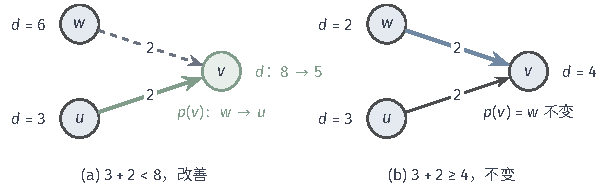
\includegraphics[width=102.993mm]{figures/01-basic-mathematics/04-graphs/tikz/c3-relaxation/figure.pdf}
  \caption{对弧$u\to v$松弛（顶点旁为当前标签，弧旁为长度）。(a) 候选值$d(u)+\ell_{u,v}=3+2=5$小于原标签$8$，标签改为$5$，前驱由$w$改为$u$（绿色表示被改善的标签与新的前驱弧，虚线为被替换的旧前驱弧）。(b) 原标签为$4$，候选值$5$不能改善，标签与前驱都不变。}
  \label{fig:graph-opt-relaxation}
\end{figure}

\paragraph{局部等式不能单独确定距离}
若没有可达负环，真实距离满足一组局部等式：$\delta(s)=0$，并且对每个可达的$v\neq s$，有$\delta(v)=\min_{u\to v}\{\delta(u)+\ell_{u,v}\}$。这只是说最短路的最后一条弧总来自某个前驱。但满足这组等式的数组不一定就是距离。设$s\to a$长$5$，$a\to b$与$b\to a$长都为$0$，则对任意$c\leq5$，取$D(s)=0$、$D(a)=D(b)=c$都满足
\[
  D(a)=\min\{D(s)+5,\ D(b)+0\}=c,\qquad D(b)=D(a)+0=c,
\]
而真实距离是$\delta(a)=\delta(b)=5$。这里的零成本环让$a,b$互相“支撑”着一个过低的值，却没有任何实际路线达到它。所以算法不能只去求解局部等式，而要从“源为零、其余为无穷”的初值出发，只沿实际路线下调标签，上面的不变量保证了这一点。初值保证标签不会无中生有，松弛保证每个标签都有路线见证，而松弛按什么次序进行、何时可以停止，则由各算法分别规定。

\paragraph{距离、前驱与访问状态}
算法通常维护三类数组，它们承担不同的职责。距离数组记录当前上界；前驱数组记录达到这个上界的最后一条弧，用于事后恢复路线；访问状态则记录算法自身的进度，例如Dijkstra算法中哪些顶点已经永久确定。前驱数组只在标签不再变化以后才能放心回溯。在一般有环图中，计算中途的前驱指针可能尚未形成从$s$出发的树；若存在可达负环，前驱指针甚至可能首尾相接成环。对于后面按轮次定义的递推，前驱还应与相应的轮次一同保存，才能把它们当作可回溯的路线。

\subsection{有向无环图上的最短路}
\label{sec:graph-opt-dag-shortest-path}

在一般的图中，一个顶点的标签可能在它的出弧已被松弛之后才下降，这时它的后继也必须随之更新。有向无环图没有这个问题：第~\ref{sec:graph-topological-order}节说明，有限有向无环图存在拓扑序，使每条弧的起点排在终点之前。按拓扑序处理顶点，轮到$v$时，所有指向$v$的弧都已被松弛，$v$的标签此后不会再变。

\begin{algorithm}[有向无环图上的最短路]
\label{alg:graph-opt-dag-shortest-path}
输入：有限有向无环图、弧长$\ell_{u,v}\in\mathbb R$、源点$s$。输出：全部距离$\delta(v)$与前驱$p(v)$。
\begin{enumerate}
  \item 求一个拓扑序$v_1,\ldots,v_n$；令$d(s)=0$，其余$d(v)=+\infty$，前驱为空。
  \item 按$i=1,\ldots,n$的顺序处理$v_i$：若$d(v_i)<+\infty$，对其每条出弧$v_i\to w$执行松弛。
  \item 对标签有限的顶点，沿前驱从终点退回$s$再反转，得到一条最短路；标签为$+\infty$的顶点报告不可达。
\end{enumerate}
\end{algorithm}

\paragraph{算例}
取弧$s\to a$长$2$、$s\to b$长$5$、$a\to b$长$-1$、$a\to t$长$5$、$b\to t$长$2$，它没有有向环，拓扑序可取$(s,a,b,t)$。处理$s$时，$a$的标签由$+\infty$改为$2$，$b$的标签由$+\infty$改为$5$。处理$a$时，候选$2+(-1)=1<5$使$b$改为$1$，同时$t$由$+\infty$改为$2+5=7$。处理$b$时，候选$1+2=3<7$使$t$改为$3$。最后处理$t$，它没有出弧。前驱为$p(a)=s$、$p(b)=a$、$p(t)=b$，从$t$回溯得到最短路$s\to a\to b\to t$，成本$2-1+2=3$。图~\ref{fig:graph-opt-dag-labels}记录了这个过程中各标签的变化。

\begin{figure}[!htb]
  \centering
  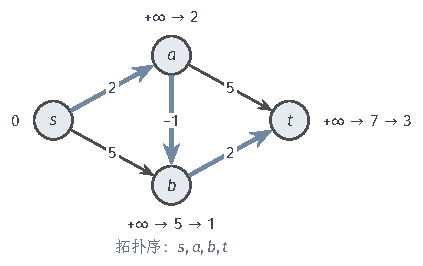
\includegraphics[width=71.635mm]{figures/01-basic-mathematics/04-graphs/tikz/c3-dag-labels/figure.pdf}
  \caption{按拓扑序$(s,a,b,t)$在有向无环图上松弛。顶点旁列出标签的变化次序，例如$b$先由处理$s$得到$5$，再由处理$a$改为$1$；蓝色粗弧是最终前驱弧，组成最短路$s\to a\to b\to t$（成本$3$）。负长度弧$a\to b$并不妨碍计算，因为正确性只依赖无环次序。}
  \label{fig:graph-opt-dag-labels}
\end{figure}

\paragraph{正确性}
上面的过程之所以能一遍完成，是因为处理到某个顶点时，所有可能到达它的路线都已考虑过。下面把这一点写成归纳证明。

\begin{theorem}[有向无环图上最短路的正确性]
\label{thm:graph-opt-dag-shortest-path}
设$\mathcal G$是有限有向无环图，弧长为任意实数。算法~\ref{alg:graph-opt-dag-shortest-path}结束时，对每个顶点$v$都有$d(v)=\delta(v)$；其中$\delta(v)=+\infty$当且仅当$v$从$s$不可达，其余$\delta(v)$均为有限值。
\end{theorem}

\begin{proof}
有向无环图中的行走不会重复顶点，因此每条行走都是简单路径，只有有限条，$\delta(v)$只可能是$+\infty$或有限值。松弛只改变弧终点的标签，而指向$v$的弧都从拓扑序中排在$v$之前的顶点出发，所以轮到$v$时它的标签已经不再改变。下面对拓扑序归纳，证明轮到$v$时$d(v)=\delta(v)$。

排在$s$之前的顶点从$s$不可达，它们的标签保持$+\infty$，与距离一致。对$v=s$，不存在回到$s$的非零步行走，故$\delta(s)=0=d(s)$。设$v$排在$s$之后，并且此前的顶点都已满足结论。若$v$不可达，则它的标签不可能变为有限值，因为有限标签总对应一条实际行走。若$v$可达，任取一条$s$到$v$的路径，设其最后一条弧为$u\to v$，则$u$排在$v$之前，路径前缀的成本不小于$\delta(u)$，归纳假设给出$\delta(u)=d(u)$。处理$u$时弧$u\to v$已被松弛，因而
\[
  d(v)\leq d(u)+\ell_{u,v}=\delta(u)+\ell_{u,v}\leq\text{该路径的成本}.
\]
路径是任取的，所以$d(v)\leq\delta(v)$。结合标签不变量$d(v)\geq\delta(v)$，得$d(v)=\delta(v)$。
\end{proof}

证明中只用到“前驱先于后继处理”，没有用到边长的符号，所以负长度弧不会造成任何问题。求拓扑序需要$O(n+a)$时间，之后每个顶点处理一次、每条弧松弛一次，总时间为$O(n+a)$，标签、前驱与拓扑序共占$O(n)$额外空间。

\paragraph{扩展示例：编辑距离}
许多递推问题的状态之间天然形成有向无环图，这时就是本小节的最短路问题。比较两段序列时，常问把序列$\bm a=(a_1,\ldots,a_p)$改写成$\bm b=(b_1,\ldots,b_q)$最少需要多少次单元素操作，允许的操作是插入一个元素、删除一个元素和把一个元素替换为另一个。以$(i,j)$表示“已把$\bm a$的前$i$个元素改写成$\bm b$的前$j$个元素”这一状态，最后一步只有三种可能：删去$a_i$，从$(i-1,j)$而来，成本为$1$；插入$b_j$，从$(i,j-1)$而来，成本为$1$；让$a_i$对应$b_j$，从$(i-1,j-1)$而来，相同时成本为$0$，不同时为一次替换，成本为$1$。于是最少操作数$E(i,j)$满足
\begin{equation}
  E(i,j)=\min\bigl\{E(i-1,j)+1,\ E(i,j-1)+1,\ E(i-1,j-1)+\mathbb I\{a_i\neq b_j\}\bigr\},
  \label{eq:graph-opt-edit-distance}
\end{equation}
边界为$E(i,0)=i$、$E(0,j)=j$，其中$\mathbb I\{\cdot\}$在条件成立时取$1$、否则取$0$。

每条状态弧都使$i+j$增加，所以状态图没有有向环，$E(p,q)$就是从$(0,0)$到$(p,q)$的最短路距离，称为两段序列的\term{编辑距离}（edit distance）。按$i+j$递增或逐行的顺序计算，正是在按拓扑序松弛。例如$\bm a=(A,B)$、$\bm b=(A,C,B)$时，三行表值依次为$(0,1,2,3)$、$(1,0,1,2)$、$(2,1,1,1)$，沿“匹配$A$、插入$C$、匹配$B$”得到距离$1$。全表连同前驱需要$O(pq)$时间与空间；只要距离值时保留相邻两行即可。更一般的序列对齐与动态时间规整留到信号与序列的应用部分，这里只说明它们的计算骨架是有向无环图上的最短路。

\subsection{Bellman--Ford算法}
\label{sec:graph-opt-bellman-ford}

图中有环时没有拓扑序可用：一个顶点的标签可能在它的出弧已被松弛之后才下降，一遍扫描不够。最直接的补救是反复扫描全部弧，直到标签不再变化。为了说清楚每一轮扫描得到了什么，先讲各轮彼此分开的同步版本。

\paragraph{同步递推}
令$d^{(0)}(s)=0$，其余$d^{(0)}(v)=+\infty$。第$k$轮只读取上一轮的标签，对每个顶点比较“沿用旧值”与“在上一轮的某条路线后再接一条弧”：
\begin{equation}
  d^{(k)}(v)=\min\Bigl\{d^{(k-1)}(v),\ \min_{u\to v}\bigl(d^{(k-1)}(u)+\ell_{u,v}\bigr)\Bigr\},\qquad k=1,2,\ldots,
  \label{eq:graph-opt-bellman-ford}
\end{equation}
没有入弧时内层最小值取$+\infty$。实现上，每轮先复制上一轮的标签数组，再逐弧用旧数组计算候选值、更新新数组。这样定义的标签有一个清楚的含义。

\begin{lemma}[同步标签的含义]
\label{lem:graph-opt-bellman-ford-k-arcs}
对每个$k\geq0$与每个顶点$v$，$d^{(k)}(v)$等于从$s$到$v$、至多含$k$条弧的全部行走的最小成本；没有这样的行走时为$+\infty$。
\end{lemma}

\begin{proof}
对$k$归纳。$k=0$时，至多零条弧的行走只有$s$处的零步行走，与$d^{(0)}$一致。设结论对$k-1$成立。一条至多含$k$条弧、到达$v$的行走，要么至多含$k-1$条弧，其成本不小于$d^{(k-1)}(v)$；要么恰含$k$条弧，去掉最后一条弧$u\to v$后剩下至多$k-1$条弧、到达$u$的前缀，其成本不小于$d^{(k-1)}(u)+\ell_{u,v}$。所以全部候选的最小值不小于式~\eqref{eq:graph-opt-bellman-ford}的右端。反过来，右端每一项都由归纳假设对应一条至多$k$条弧的行走，最小值能够达到。故两者相等。
\end{proof}

沿用上一小节的四点图，并把它看成一般的有向图，按式~\eqref{eq:graph-opt-bellman-ford}逐轮计算，结果见表~\ref{tab:graph-opt-bellman-ford-rounds}。第$1$轮只能用一条弧，得到$a=2$、$b=5$；第$2$轮允许两条弧，$b$经$a$降到$1$，$t$经$a$得到$7$；第$3$轮$t$经$b$降到$3$；第$4$轮不再变化。每一列恰好是“至多$k$条弧”的最优值，例如$d^{(2)}(t)=7$对应两弧路线$s\to a\to t$，而三弧路线$s\to a\to b\to t$要到第$3$轮才被计入。

\begin{table}[!htb]
  \centering
  \caption{同步Bellman--Ford在四点图（$s\to a$长$2$，$s\to b$长$5$，$a\to b$长$-1$，$a\to t$长$5$，$b\to t$长$2$）上的逐轮标签。第$k$行是至多$k$条弧的最小成本，括号内为该轮改变标签时的前驱。}
  \label{tab:graph-opt-bellman-ford-rounds}
  \begin{tabular}{ccccc}
    \toprule
    轮次$k$ & $d^{(k)}(s)$ & $d^{(k)}(a)$ & $d^{(k)}(b)$ & $d^{(k)}(t)$ \\
    \midrule
    $0$ & $0$ & $+\infty$ & $+\infty$ & $+\infty$ \\
    $1$ & $0$ & $2$（$s$） & $5$（$s$） & $+\infty$ \\
    $2$ & $0$ & $2$ & $1$（$a$） & $7$（$a$） \\
    $3$ & $0$ & $2$ & $1$ & $3$（$b$） \\
    $4$ & $0$ & $2$ & $1$ & $3$ \\
    \bottomrule
  \end{tabular}
\end{table}

\paragraph{轮数上界与就地更新}
需要多少轮？对不受可达负环影响的顶点$v$，第~\ref{sec:graph-opt-path-cost}节说明$\delta(v)$由一条简单路径达到，而简单路径至多经过$n$个顶点、含$n-1$条弧。由引理~\ref{lem:graph-opt-bellman-ford-k-arcs}，第$n-1$轮已经计入这条路径，所以$d^{(n-1)}(v)=\delta(v)$。若某一整轮没有任何标签改变，则此后各轮的输入都相同，标签不会再变，可以提前停止；四点图在第$4$轮发现无改善，实际只需$3$轮。

常见的实现不复制数组，而是在同一个数组上逐弧松弛，一轮中刚改善的标签可以立即被同一轮后面的弧使用，称为就地更新。按$s\to a$、$s\to b$、$a\to b$、$a\to t$、$b\to t$的顺序扫描四点图，第一轮就得到全部最终标签$(0,2,1,3)$。就地更新得到的标签仍是真实行走的成本，又对每轮都不高于同步版本的标签（对轮数归纳即可），所以$n-1$轮的上界照样成立。但“第$k$轮标签恰为至多$k$条弧的最优值”这一解释只属于同步版本，不能原样套在就地更新上：同一轮内的改善可能已经串起了多条弧。

\paragraph{负环影响的检测与传播}
完成$n-1$轮以后，不受负环影响的顶点已经得到正确距离，剩下的问题是找出哪些顶点的距离为$-\infty$。固定此时的标签$d=d^{(n-1)}$，检查所有满足$d(u)<+\infty$且$d(u)+\ell_{u,v}<d(v)$的弧$u\to v$，即再做一轮仍能改善的弧，把它们的终点称为种子。然后从全部种子出发，沿出弧做一次遍历，把遍历到的顶点都标记为$-\infty$。

\begin{theorem}[Bellman--Ford算法对三类结果的判定]
\label{thm:graph-opt-bellman-ford-negative-cycles}
在同步递推的$n-1$轮之后按上述方法标记，被标记的顶点恰好是$\delta(v)=-\infty$的顶点；其余顶点中，$d^{(n-1)}(v)=+\infty$的不可达，$d^{(n-1)}(v)$有限的满足$d^{(n-1)}(v)=\delta(v)$。
\end{theorem}

\begin{proof}
先证每个种子$v$都满足$\delta(v)=-\infty$。由引理~\ref{lem:graph-opt-bellman-ford-k-arcs}，$v$可改善说明$d^{(n)}(v)<d^{(n-1)}(v)$，即存在一条恰含$n$条弧的行走，比所有至多$n-1$条弧的行走都便宜。含$n$条弧的行走经过$n+1$个顶点位置，必有顶点重复，从中可以切出一段闭行走$C$。若$C$的成本非负，删去它会得到弧更少、成本不更高的行走，与上述“更便宜”矛盾；故$C$的成本为负，由第~\ref{sec:graph-opt-path-cost}节的分解，$C$中含有一个负环。这个负环位于一条从$s$出发、到达$v$的行走上，所以$\delta(v)=-\infty$。从种子沿出弧能到达的顶点也能从同一个负环到达，因而被标记的顶点距离都是$-\infty$。

再证每个$\delta(v)=-\infty$的顶点都会被标记。此时存在从$s$可达的负环$C=(c_0,c_1,\ldots,c_k=c_0)$能到达$v$。$C$上的顶点从$s$可达，可达顶点至多经$n-1$条弧到达，所以它们的标签有限。若$C$上没有一条弧可改善，则对每条环弧都有$d(c_{r})\leq d(c_{r-1})+\ell_{c_{r-1},c_r}$，沿环相加，两侧的标签之和恰好相消，得到$0\leq\ell(C)<0$，矛盾。因此$C$上至少有一个种子，而$v$能从$C$到达，必然被遍历标记。

最后，未被标记且可达的顶点不受任何可达负环影响，前面已说明$d^{(n-1)}(v)=\delta(v)$；不可达顶点的标签始终为$+\infty$。
\end{proof}

回到图~\ref{fig:graph-opt-distance-outcomes}。该图有$7$个顶点，同步计算$6$轮后，$u$的标签为$4$，$x,y$保持$+\infty$，而$a,b,t$的标签分别为$-3,-2,2$，这些值本身没有意义，只是绕圈到第$6$轮时恰好停留的数。此时弧$b\to a$与$b\to t$仍可改善，种子是$a$与$t$；从种子沿出弧遍历，标记出$\{a,b,t\}$。于是算法报告$u$的距离为$4$，$a,b,t$为$-\infty$，$x,y$不可达，与前面的分析一致。不受影响的旁支$u$必须保留有限答案。

\paragraph{计算开销与路径回溯}
每轮逐弧扫描一次，用时$O(a)$，至多$n-1$轮，再加上一轮检测与一次遍历，总时间为$O(na)$。同步版本每轮还要复制标签数组，另需$O(n)$时间，合计至多$O(n^2)$；就地更新省去这部分。只保存当前和上一轮的标签时，工作状态为$O(n)$；若要按引理~\ref{lem:graph-opt-bellman-ford-k-arcs}的含义回溯“至多$k$条弧”的最优路线，就需要保存每一轮的前驱$p^{(k)}(v)$，记录可达$O(n^2)$条。

只保存一份前驱数组时，也可以回溯有限距离的顶点，但要说明这份前驱与递推相容。设$v$未被标记且标签有限，若$p(v)=u$，则$u\to v$是一条弧，$u$也不会被标记，否则$v$能从负环到达。由于标签只降不升，任一时刻每条前驱弧都满足$d(p(w))+\ell_{p(w),w}\leq d(w)$。前驱指针在未标记顶点之间不会成环：若成环，考察环上最后被设置的那个指针，在它被设置之前，环上其余前驱弧都满足上述不等式，而这条弧满足严格不等式，沿环相加，标签相消，得到环的成本为负；这个负环从$s$可达，又能沿前驱弧到达$v$，与$v$未被标记矛盾。于是从$v$沿前驱必能回到$s$。把沿途的不等式相加，所得路线的成本不超过$d(v)=\delta(v)$，因而恰好是一条最短路。对标为$-\infty$的顶点，算法给出的不是一条“最短路”，而是负环的证据：一个种子、一条从$s$到负环的行走与一条从负环到该顶点的行走。

\subsection{Dijkstra算法}
\label{sec:graph-opt-dijkstra}

Bellman--Ford算法要反复扫描全部弧，因为一个标签随时可能再被改小。若边长都非负，情况就不同了：在尚未确定的顶点中，标签最小的那个已经不可能再被改小，因为任何绕道而来的路线都要先经过某个标签不更小的顶点，后半程又不会让成本下降。Dijkstra算法利用这一点，每次永久确定一个顶点。

\paragraph{适用条件与算法步骤}
Dijkstra算法要求从源点可达部分的弧长都非负。全图非负是便于检查的充分条件；从$s$到达不了的区域即使有负边，也不影响本次查询。在这一条件下，从$s$可达的部分不含负环，所有距离都是$+\infty$或有限值。

\begin{algorithm}[Dijkstra算法]
\label{alg:graph-opt-dijkstra}
输入：有限有向图、源点$s$，从$s$可达部分的弧长非负。输出：全部距离$\delta(v)$与前驱$p(v)$。状态：标签$d$、前驱$p$、已确定集合$R$，以及按标签排序的未确定顶点优先队列。
\begin{enumerate}
  \item 令$d(s)=0$，其余$d(v)=+\infty$，$R=\varnothing$。
  \item 当存在标签有限的未确定顶点时，取出其中标签最小的$u$，把$u$加入$R$。
  \item 对$u$的每条出弧$u\to v$，若$v\notin R$，执行松弛；标签改善时更新优先队列中$v$的键。
  \item 结束时，$R$中顶点的标签即为距离，其余顶点不可达。
\end{enumerate}
\end{algorithm}

优先队列有两种常见实现。一种是支持“降键”的索引堆，每个顶点在堆中只有一个条目，标签改善时原地下调它的键。另一种不降键，标签改善时直接插入一个新条目$(d(v),v)$，旧条目留在堆中；出队时若发现该顶点已在$R$中，说明这是过期条目，直接丢弃。两种实现的输出相同，区别只在队列规模与操作次数。

\paragraph{为什么出队时标签已经正确}
算法的关键论断是：顶点被加入$R$的那一刻，它的标签已经等于真实距离，此后不再需要修正。证明的切入点是一条假设更短的路线上第一个尚未确定的顶点。

\begin{theorem}[Dijkstra算法的正确性]
\label{thm:graph-opt-dijkstra}
若从$s$可达部分的弧长都非负，则算法~\ref{alg:graph-opt-dijkstra}中每个顶点$u$被加入$R$时都有$d(u)=\delta(u)$；算法结束时未加入$R$的顶点从$s$不可达。
\end{theorem}

\begin{proof}
对加入$R$的次序归纳。第一个加入的是$s$，$d(s)=0=\delta(s)$，因为可达部分没有负环。设此前加入$R$的顶点都满足$d=\delta$，现在$u$被选出，且$d(u)<+\infty$。由标签不变量，$d(u)\geq\delta(u)$。假设$d(u)>\delta(u)$，取一条$s$到$u$、成本为$\delta(u)$的简单路径$P$。$P$从$s\in R$出发，到达$u\notin R$，所以沿$P$存在第一个不在$R$中的顶点$y$，记它在$P$上的前一个顶点为$x\in R$。

$x$加入$R$时弧$x\to y$已被松弛，此后标签只会下降，所以$d(y)\leq d(x)+\ell_{x,y}$。归纳假设给出$d(x)=\delta(x)$；而最短路的前缀仍是最短路，故$\delta(x)+\ell_{x,y}=\delta(y)$。于是$d(y)\leq\delta(y)$。$P$从$y$到$u$的后半段由可达部分的弧组成，长度非负，因而$\delta(y)\leq\delta(u)$。合起来得到
\[
  d(y)\leq\delta(y)\leq\delta(u)<d(u).
\]
但$y$也是未确定顶点，而算法选出的$u$在未确定顶点中标签最小，应有$d(u)\leq d(y)$，矛盾。所以$d(u)=\delta(u)$。

若算法停止时某个可达顶点$v$不在$R$中，取一条$s$到$v$的路径，同样找出第一个不在$R$中的顶点$y$及其前驱$x\in R$。松弛$x\to y$已使$d(y)$有限，算法便不会在此时停止，矛盾。
\end{proof}

\paragraph{负边反例}
证明中只有一步用到非负性：“后半段长度非负，所以$\delta(y)\leq\delta(u)$”。这一步失效时，算法确实会出错，即使图中没有负环。取弧$s\to a$长$2$、$s\to b$长$5$、$b\to a$长$-4$，如图~\ref{fig:graph-opt-dijkstra-counterexample}。处理$s$后，$a$的标签为$2$、$b$为$5$；算法选出标签较小的$a$并永久确定$d(a)=2$。随后处理$b$时，候选$5+(-4)=1$本可改善$a$，但$a$已在$R$中，不再更新。真实距离是$\delta(a)=1$，由路线$s\to b\to a$达到。对照证明，这里的$y=b$、$u=a$，后半段$b\to a$为负，使$\delta(b)=5>\delta(a)=1$，“首个未确定顶点的标签不超过$\delta(u)$”不再成立。

\begin{figure}[!htb]
  \centering
  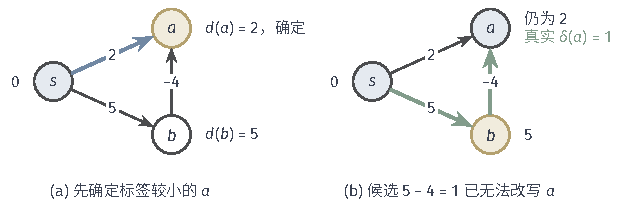
\includegraphics[width=105.583mm]{figures/01-basic-mathematics/04-graphs/tikz/c3-dijkstra-counterexample/figure.pdf}
  \caption{负边使Dijkstra算法过早确定标签。(a) 处理$s$后，$a$的标签$2$小于$b$的标签$5$，$a$被永久确定（黄色为当前出队顶点）。(b) 处理$b$时候选值$5-4=1$已无法改写$a$；真实最短路是$s\to b\to a$（绿色），成本$1$。图中没有负环，出错的原因是后半段弧$b\to a$为负。}
  \label{fig:graph-opt-dijkstra-counterexample}
\end{figure}

\paragraph{出队轨迹}
把四点图中$a\to b$的长度由$-1$改为$1$，全部弧长非负，Dijkstra算法适用。下面依次列出出队顶点与松弛结果：
\begin{enumerate}
  \item 取出$s$（标签$0$），松弛得$d(a)=2$、$d(b)=5$，前驱都是$s$；
  \item 取出$a$（标签$2$），候选$2+1=3<5$使$d(b)=3$、$p(b)=a$，候选$2+5=7$使$d(t)=7$、$p(t)=a$；
  \item 取出$b$（标签$3$），候选$3+2=5<7$使$d(t)=5$、$p(t)=b$；
  \item 取出$t$（标签$5$），没有出弧，队列为空。
\end{enumerate}
最终$\delta(a)=2$、$\delta(b)=3$、$\delta(t)=5$，从$t$沿前驱回溯得到$s\to a\to b\to t$。图~\ref{fig:graph-opt-dijkstra-trace}画出每次出队后的状态：已确定集合$R$逐个向外扩张，每个顶点在出队时的标签都不再改变。

\begin{figure*}[!htb]
  \centering
  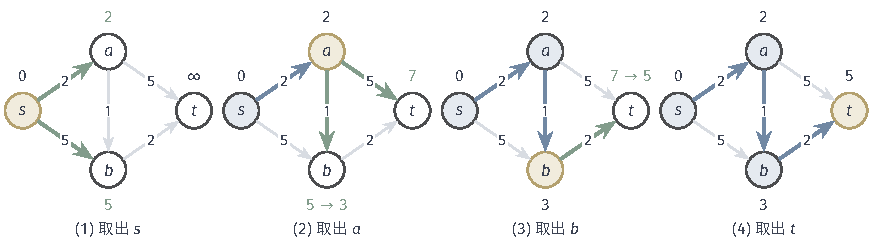
\includegraphics[width=147.687mm]{figures/01-basic-mathematics/04-graphs/tikz/c3-dijkstra-trace/figure.pdf}
  \caption{Dijkstra算法在非负四点图上的出队过程（$a\to b$长$1$，其余同前）。每个面板对应一次出队：蓝色为已确定顶点，黄色为本次出队的顶点，绿色标签与绿色弧表示本次松弛改善的标签及新前驱。四次出队依次确定$s=0$、$a=2$、$b=3$、$t=5$，最终前驱弧组成路线$s\to a\to b\to t$。}
  \label{fig:graph-opt-dijkstra-trace}
\end{figure*}

\paragraph{计算开销}
每个顶点至多出队一次，每条弧在其起点出队时松弛一次。用邻接表存储图、用支持降键的索引二叉堆存储未确定顶点时，取最小与降键各需$O(\log n)$时间，总时间为$O((n+a)\log n)$；标签、前驱、堆及其位置索引共占$O(n)$额外空间，图本身的存储另计。不降键的实现每次改善插入一个条目，堆中至多有$a+1$个条目，操作时间为$O(\log a)=O(\log n)$，总时间仍为$O((n+a)\log n)$，但队列空间上界变为$O(a)$。稠密图上也可以不用堆，每次扫描数组找最小标签，总时间为$O(n^2+a)$。

\subsection{方法比较与结果检验}
\label{sec:graph-opt-shortest-path-comparison}

三种算法解决同一个单源问题，但对输入的要求不同。比较它们时应先问：图有没有有向环？可达部分有没有负长度弧？是否需要检测负环？然后才比较运行时间。表~\ref{tab:graph-opt-shortest-path-methods}汇总了这些区别。

\begin{table}[!htb]
  \centering
  \caption{三种单源最短路算法的比较（$n$为顶点数，$a$为弧数，邻接表存储）。}
  \label{tab:graph-opt-shortest-path-methods}
  \begin{tabular}{llll}
    \toprule
    & 有向无环图递推 & Bellman--Ford & Dijkstra \\
    \midrule
    图结构 & 无有向环 & 不限 & 不限 \\
    弧长 & 任意实数 & 任意实数 & 可达部分非负 \\
    标签修正 & 处理后不变 & 反复修正 & 出队后不变 \\
    负环 & 不会出现 & 检测并标记 & 条件排除 \\
    时间 & $O(n+a)$ & $O(na)$ & $O((n+a)\log n)$ \\
    正确性依据 & 拓扑序归纳 & 至多$k$弧递推 & 首个未定顶点 \\
    \bottomrule
  \end{tabular}
\end{table}

“允许负边”与“存在负环”是两件不同的事。有向无环图递推与Bellman--Ford算法都允许负边；前者因为无环而不会遇到负环，后者则能在负环存在时正确报告受影响的顶点。Dijkstra算法连负边都不允许，哪怕负边并不构成负环，图~\ref{fig:graph-opt-dijkstra-counterexample}就是这样的例子。一种算法在某组数据上跑得更快、甚至答案碰巧正确，都不能替代对其条件的检查。

\paragraph{有限距离的检验}
拿到一份声称的最短路结果后，可以不重跑算法而直接核对。对标签有限的顶点，先沿前驱恢复路线，检查起点为$s$、终点为$v$、每一步都是原图中的弧，并重算弧长之和是否等于$d(v)$。这一步证明标签可以达到，即$d(v)\geq\delta(v)$。

最优性需要反方向的下界。若输出满足$d(s)=0$，并且对每条起点标签有限的弧$u\to v$都有
\[
  d(v)\leq d(u)+\ell_{u,v},
\]
那么任取一条$s$到$v$的行走$W=(s=w_0,w_1,\ldots,w_k=v)$，沿$W$把这些不等式逐条相加，中间标签相消，得到$d(v)\leq d(s)+\ell(W)=\ell(W)$。所以$d(v)\leq\delta(v)$，与可达性一起给出$d(v)=\delta(v)$。这组逐弧不等式只需$O(n+a)$时间核对，它本身就是有限距离的最优性证书；不满足时，违反不等式的弧直接指出了一条更好的路线。

\paragraph{不可达与负无穷的检验}
另外两类结果需要不同的证据。对报告为$+\infty$的顶点，用一次广度优先遍历核对它确实不在$s$的可达集中。对报告为$-\infty$的顶点，应给出三段证据：一条从$s$到某个有向环的行走、该环的成本为负，以及一条从环到该顶点的行走。三类结果各有各的验收方式，不能只核对其中一类就宣布整份结果正确。

% 第3章第2节：最小生成树（问题与最短路树的区别、割性质与安全选边、Kruskal、Prim、方法比较与结果检验）。

\section{最小生成树}
\label{sec:graph-minimum-spanning-tree}

要在若干城镇之间修路，使任意两个城镇都能互相到达，每条候选道路都有建造成本。这时关心的不是某两点之间怎样走最近，而是整张网络的总造价。第~\ref{sec:graph-trees-forests}节说明，连通且无环的边集恰好连接全部顶点而没有多余的边，即生成树；多一条边便形成环，环上任意一条边都可以拆掉而不破坏连通。于是问题化为：在所有生成树中找总边权最小的一棵。

本节先给出问题并与最短路区分，再建立割性质，它说明怎样的边可以放心地选入。Kruskal算法与Prim算法以不同的方式维护当前选边，但每一步都由割性质保证安全。最后在同一算例上比较两种算法，并区分“结果是一棵生成树”与“结果是最优的”这两种检查。

\subsection{最小生成树问题}
\label{sec:graph-opt-mst-problem}

设$\mathcal G=(V,E)$是有限无向连通图，每条边$e$带有实数权$w_e$，表示建造成本。对生成树$T\subseteq E$，记其总成本为$w(T)=\sum_{e\in T}w_e$。

\begin{definition}[最小生成树]
\label{def:graph-opt-mst}
有限无向连通加权图的所有生成树中，总成本$w(T)$最小者称为\term{最小生成树}（minimum spanning tree）。
\end{definition}

生成树只有有限多棵，所以最小生成树总是存在。它最小化的是连接全部顶点的总成本，并不保证树上每对顶点之间的路线都是原图中的最短路。图~\ref{fig:graph-opt-mst-vs-spt}中，三角形三条边的权为$w_{x,y}=2$、$w_{y,z}=2$、$w_{x,z}=3$。最小生成树取$\{xy,yz\}$，成本$4$；但在树上$x$到$z$要绕经$y$，长度为$4$，而原图中的直达边只有$3$。以$x$为源的\term{最短路树}（shortest-path tree），即由各顶点最短路的前驱弧组成的树，是$\{xy,xz\}$，成本$5$。两者回答不同的问题，一般不相同。同样，第~\ref{sec:graph-connectivity-computation}节由遍历得到的生成森林只保证连通与无环，不带有任何成本上的最优性。

\begin{figure}[!htb]
  \centering
  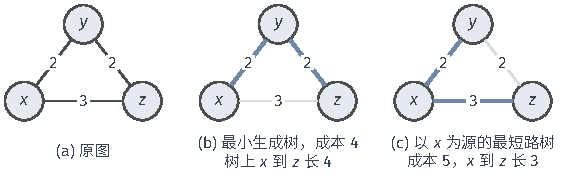
\includegraphics[width=95.793mm]{figures/01-basic-mathematics/04-graphs/tikz/c3-mst-vs-spt/figure.pdf}
  \caption{最小生成树与最短路树可以不同。(a) 原图，边旁为权。(b) 最小生成树$\{xy,yz\}$总成本$4$，但树上$x$到$z$的路线长$4$。(c) 以$x$为源的最短路树$\{xy,xz\}$保证每个顶点到$x$的距离最短，总成本却是$5$。蓝色粗边为所选的边。}
  \label{fig:graph-opt-mst-vs-spt}
\end{figure}

\paragraph{非连通、负权与平局}
图不连通时不存在生成树，问题改为在每个连通分量内分别求最小生成树，合起来称为\term{最小生成森林}（minimum spanning forest）。负权不会带来最短路那样的困难：每棵生成树恰有$n-1$条边，把所有边权同时加上常数$c$，每棵生成树的成本都增加$(n-1)c$，比较结果不变，因此总可以设想权都为正。边权有相同值时，最小生成树可能不止一棵，但最小总成本是唯一的。若要最大化总权，把全部边权取负即化为最小化问题，得到\term{最大生成树}（maximum spanning tree），下面的割性质与两种算法只需把“最小”改为“最大”即可照用。第~\ref{sec:graph-tree-decomposition-construction}节构造团树时会用到最大生成树。

\subsection{割性质与安全选边}
\label{sec:graph-opt-cut-property}

两种算法都是逐条选边，并希望每一步都不走错。“不走错”的确切含义是：当前已选的边集$A$总能扩充成某一棵最小生成树。只要保持这个不变量，选满$n-1$条边时，$A$本身就是一棵最小生成树。问题在于，下一条边选哪条才能保持不变量。

\paragraph{割与轻边}
把顶点集分成两个非空部分$S$与$V\setminus S$，称为图的一个\term{割}（cut），记作$(S,V\setminus S)$。一条边的两个端点分别在两侧时，称它跨越这个割。若已选边集$A$中没有边跨越该割，就称这个割与$A$相容。跨越某个割的边中权最小的称为该割的\term{轻边}（light edge），权相同时轻边可以不止一条。

\begin{lemma}[割性质]
\label{lem:graph-opt-cut-property}
设$\mathcal G$是有限无向连通加权图，边集$A$包含在某棵最小生成树中，割$(S,V\setminus S)$与$A$相容，$e$是该割的一条轻边。则$A\cup\{e\}$也包含在某棵最小生成树中。
\end{lemma}

\begin{proof}
取一棵包含$A$的最小生成树$T$。若$e\in T$，结论已成立。否则把$e$加入$T$，由第~\ref{sec:graph-trees-forests}节，树加一条边恰好形成一个环。设$e=\{u,v\}$，$u\in S$、$v\notin S$，这个环由$e$与$T$中$u$到$v$的路径组成。这条路径从$S$出发，最终到达$V\setminus S$，所以其中至少有一条边$f$跨越该割。

从$T+e$中删去$f$，环被打断，所得边集$T'=T+e-f$仍连通且有$n-1$条边，因而是生成树。由于$e$是轻边，$w_e\leq w_f$，所以$w(T')=w(T)+w_e-w_f\leq w(T)$，$T'$也是最小生成树。最后，割与$A$相容，跨越割的$f$不在$A$中，删去$f$不影响$A$；于是$A\cup\{e\}\subseteq T'$。
\end{proof}

图~\ref{fig:graph-opt-cut-exchange}画出这一交换：轻边$e$加入后与树中路径形成环，环上另一条跨割边$f$被删去，成本不增。

\begin{figure}[!htb]
  \centering
  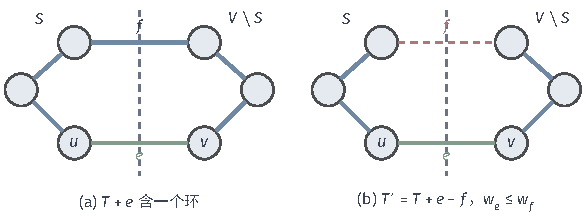
\includegraphics[width=99.187mm]{figures/01-basic-mathematics/04-graphs/tikz/c3-cut-exchange/figure.pdf}
  \caption{割性质的交换论证。虚线把顶点分成$S$与$V\setminus S$，蓝色粗边为最优树$T$，其中不跨割的边包含当前选边$A$。(a) 轻边$e$（绿色）不在$T$中，加入后与$T$中$u$到$v$的路径形成环。(b) 环上另一条跨割边$f$（红色虚线）被删去，得到$T'=T+e-f$，因$w_e\leq w_f$，成本不增。}
  \label{fig:graph-opt-cut-exchange}
\end{figure}

\paragraph{安全不等于必选}
割性质只保证轻边能留在\emph{某一棵}最优树中，并不保证它出现在\emph{每一棵}最优树中。设三角形三条边的权都是$1$，取割$(\{x\},\{y,z\})$，$xy$与$xz$都是轻边。最小生成树$\{xy,yz\}$不含$xz$，但按割性质选入$xz$仍然安全，因为$\{xz,yz\}$同样是最小生成树。平局时不同的选择通向不同的最优树，最优成本却相同。

割性质是两种算法的共同依据，区别只在于它们选取哪个割：Kruskal算法以当前森林中某个分量作为$S$，Prim算法以当前唯一一棵树的顶点集作为$S$。

\subsection{Kruskal算法}
\label{sec:graph-opt-kruskal}

一种自然的想法是从最便宜的边开始逐条考虑，只要不形成环就选入。开始时每个顶点自成一个分量；一条边的两端若属于不同分量，选入它会把两个分量连起来，不会成环；若两端已在同一分量，选入它就会成环，应当跳过。

\begin{algorithm}[Kruskal算法]
\label{alg:graph-opt-kruskal}
输入：有限无向加权图。输出：最小生成森林的边集$A$。状态：已选边集$A$与维护当前分量的并查集。
\begin{enumerate}
  \item 令$A=\varnothing$，为每个顶点建立一个单元素集合；把全部边按权从小到大排序，平局按固定的边序。
  \item 按排序依次取边$\{u,v\}$：若$u,v$的代表不同，把这条边加入$A$并合并两个集合；若代表相同，跳过。
  \item 选满$n-1$条边时可提前停止；否则扫描完全部边，输出的$A$是最小生成森林，集合个数即连通分量数。
\end{enumerate}
\end{algorithm}

判断两端是否属于同一分量、以及合并两个分量，正是第~\ref{sec:graph-connectivity-computation}节并查集的find与union操作。每选一条边，分量数减一且不产生环，所以选边数加分量数始终等于$n$。

\paragraph{算例}
取五个顶点$a,b,c,d,e$与七条边，权为$ab=1$、$bc=2$、$cd=3$、$ac=4$、$bd=5$、$ce=6$、$de=7$。按权依次考虑：$ab$、$bc$、$cd$的两端都属于不同分量，依次选入，此时分量为$\{a,b,c,d\}$与$\{e\}$，累计成本$6$；$ac$与$bd$的两端都已在$\{a,b,c,d\}$中，选入会成环，跳过；$ce$连接两个分量，选入后只剩一个分量，已选满$4=n-1$条边，停止。结果为$\{ab,bc,cd,ce\}$，总成本$1+2+3+6=12$。图~\ref{fig:graph-opt-kruskal-steps}画出了这一过程。这个图共有$21$棵生成树，逐一枚举可以核对成本$12$的只有这一棵，次优的成本为$13$。

\begin{figure}[!htb]
  \centering
  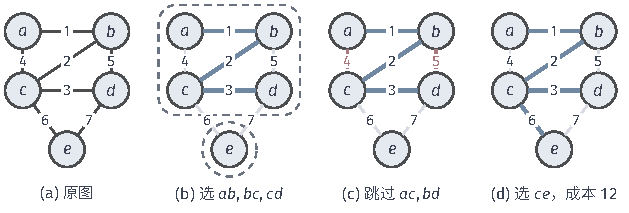
\includegraphics[width=106.5mm]{figures/01-basic-mathematics/04-graphs/tikz/c3-kruskal-steps/figure.pdf}
  \caption{Kruskal算法在五点七边图上的过程。(a) 原图，边旁为权。(b) 依次选入$ab,bc,cd$（蓝色粗边），虚线框标出当前分量$\{a,b,c,d\}$与$\{e\}$。(c) $ac$与$bd$的两端已在同一分量，选入会成环，跳过（红色虚线）。(d) 选入$ce$，得到最小生成树$\{ab,bc,cd,ce\}$，总成本$12$。}
  \label{fig:graph-opt-kruskal-steps}
\end{figure}

\paragraph{正确性}
下面用割性质说明Kruskal算法每次选入的边都是安全的。

\begin{theorem}[Kruskal算法的正确性]
\label{thm:graph-opt-kruskal}
对有限无向加权图，算法~\ref{alg:graph-opt-kruskal}输出一个最小生成森林；图连通时输出最小生成树。
\end{theorem}

\begin{proof}
先设图连通，证明不变量“$A$包含在某棵最小生成树中”。初始$A=\varnothing$，结论成立。设算法即将选入边$e=\{u,v\}$，取$S$为森林$(V,A)$中$u$所在的分量，则$v\notin S$，割$(S,V\setminus S)$与$A$相容。考察任意一条跨越这个割、权小于$w_e$的边$g$。它排在$e$之前，已被处理过：若当时被选入，它就在$A$中，而$A$中没有跨割的边；若当时被跳过，它的两端当时已在同一分量，分量只会合并而不会拆开，现在仍在同一分量，也不能跨割。所以跨越该割的边权都不小于$w_e$，$e$是轻边，由引理~\ref{lem:graph-opt-cut-property}，选入$e$后不变量仍成立。

扫描结束时，若原图中某条边连接了$(V,A)$的两个不同分量，处理到它时两端必属不同分量，它就会被选入，矛盾。所以$(V,A)$的分量与原图的分量相同，图连通时$A$是生成树。它包含在某棵最小生成树中，又与之边数相同，因而本身就是最小生成树。图不连通时，对每个分量分别应用上面的论证，结论对最小生成森林同样成立。
\end{proof}

\paragraph{计算开销}
排序需要$O(m\log m)$时间。之后至多处理$m$条边，每条边做两次find，选入时再做一次union，共$O(m)$次并查集操作。采用第~\ref{sec:graph-connectivity-computation}节的按大小合并时，树高不超过$O(\log n)$，每次操作$O(\log n)$，这部分为$O(m\log n)$；由于$m\leq n^2$，$\log m\leq2\log n$，总时间为$O(m\log n)$，空间为边表与并查集的$O(n+m)$。若再配合路径压缩，并查集操作的摊还开销几乎为常数，此时排序成为主要开销。算法的正确性只依赖割性质，与并查集采用哪种实现无关。

\subsection{Prim算法}
\label{sec:graph-opt-prim}

Kruskal算法同时维护许多分量，按全局次序选边。另一种做法是只让一棵树生长：从一个顶点出发，每次把一个外部顶点用最便宜的边接到树上。

\paragraph{键与算法步骤}
为每个尚未入树的顶点$v$记录一个键$\operatorname{key}(v)$，表示$v$与当前树之间最便宜的边的权，同时记录这条边在树内的端点$p(v)$。这里的键是\emph{一条}连接边的权，不是Dijkstra算法中从源点出发的累计长度。

\begin{algorithm}[Prim算法]
\label{alg:graph-opt-prim}
输入：有限无向连通加权图、起点$r$。输出：最小生成树的边集。状态：树的顶点集$S$、外部顶点的键与父点、按键排序的优先队列。
\begin{enumerate}
  \item 令$S=\{r\}$；对$r$的每个邻居$v$，令$\operatorname{key}(v)=w_{r,v}$、$p(v)=r$，其余外部顶点的键为$+\infty$。
  \item 当$S\neq V$时，取出键最小的外部顶点$u$，把$u$加入$S$，把边$\{p(u),u\}$加入树。
  \item 对$u$的每个外部邻居$v$，若$w_{u,v}<\operatorname{key}(v)$，令$\operatorname{key}(v)=w_{u,v}$、$p(v)=u$。
\end{enumerate}
\end{algorithm}

第三步之后，每个外部顶点的键仍等于它与$S$中顶点之间最便宜的边权：新加入的$u$只带来了从$u$出发的边，逐一比较即可。因此每次取出的最小键对应的边，正是割$(S,V\setminus S)$的一条轻边。

\paragraph{算例}
在与Kruskal算法相同的五点图上从$a$出发，过程如图~\ref{fig:graph-opt-prim-steps}。开始时$\operatorname{key}(b)=1$、$\operatorname{key}(c)=4$。取出$b$，选入$ab$；$b$的邻边把$c$的键从$4$改为$2$，并给$d$设键$5$。取出$c$，选入$bc$；$d$的键从$5$改为$3$，$e$得到键$6$。取出$d$，选入$cd$；$de=7$不优于$e$现有的键$6$，不更新。最后取出$e$，选入$ce$。所得的树与Kruskal算法相同，成本$12$。

\begin{figure*}[!htb]
  \centering
  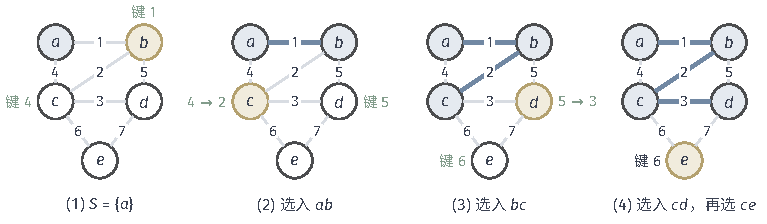
\includegraphics[width=129.858mm]{figures/01-basic-mathematics/04-graphs/tikz/c3-prim-steps/figure.pdf}
  \caption{Prim算法从$a$出发的过程。每个面板中蓝色顶点与蓝色粗边是当前树，外部顶点旁标出键，绿色表示刚被改善的键，黄色为下一个取出的顶点。依次选入$ab,bc,cd,ce$，各步加入的边恰是当前树顶点集所形成割的轻边；最终的树与Kruskal算法相同，成本$12$。}
  \label{fig:graph-opt-prim-steps}
\end{figure*}

换一个起点，选边次序会变。从$e$出发时，$c$与$d$的键分别为$6$与$7$；先选入$ec=6$，$c$的邻边使$b$、$a$、$d$的键变为$2$、$4$、$3$；再选入$cb=2$，$a$的键降为$1$；随后选入$ba=1$与$cd=3$。所选边权依次为$6,2,1,3$，并不递增。这与Kruskal算法的全局排序不同：Prim算法每次只在当前割上取最轻的边，不同时刻面对的是不同的割。

\paragraph{正确性}
正确性同样来自割性质：令$A$为当前树的边集，$S$为其顶点集。$A$的边都在$S$内部，割$(S,V\setminus S)$与$A$相容；算法选入的边是该割的轻边，由引理~\ref{lem:graph-opt-cut-property}，若$A$包含在某棵最小生成树中，加入新边后仍然如此。从$A=\varnothing$出发归纳，选满$n-1$条边时得到最小生成树。

\paragraph{实现与开销}
用数组保存键、每次线性扫描找最小时，$n$次取最小共$O(n^2)$，每条边至多引起一次键的比较与更新，总时间为$O(n^2+m)$，适合稠密图。用支持降键的索引二叉堆时，取最小与降键各需$O(\log n)$，总时间为$O((n+m)\log n)$，适合稀疏图。两种实现的额外空间都是$O(n)$。图不连通时，一棵树长满所在分量后，从任一尚未访问的顶点重新开始，得到最小生成森林，各分量的父边与成本分别保留。

\subsection{方法比较与结果检验}
\label{sec:graph-opt-mst-comparison}

两种算法读取边与维护状态的方式不同。Kruskal算法一次性对全部边排序，按全局次序检查，用并查集维护多个分量，适合边已经以列表形式给出的稀疏图。Prim算法从一棵树出发，只读取新入树顶点的邻边，用键数组或堆维护局部信息，在用邻接矩阵存储的稠密图上，数组版本的$O(n^2)$开销已与读入图的开销同阶。孰优孰劣取决于图的稠密程度、边的组织方式和所用数据结构，不能只凭算法名称判断。

\paragraph{可行性与最优性}
检验一份声称的最小生成森林时，先确认它是一个可行的生成森林：所选的每条边都来自原图；每个原连通分量的顶点都被覆盖；所选边无环，可以用并查集逐条加入核对；选边数等于$n$减去分量数。然后重算总成本。这些检查只证明结果是\emph{一个}生成森林，不能证明它最优。

最优性要回到割性质与算法的交换论证。一种可以独立执行的检查是：对每条未被选中的边$\{u,v\}$，考察树上$u$到$v$的路径，若路径上有一条边的权大于$w_{u,v}$，用这条非树边替换它，就得到成本更低的生成树，结果必不最优。反过来，若每条非树边都不轻于它在树上对应路径中的每条边，这棵树就是最优的；这一充分性可以仿照割性质的交换论证证明，这里从略。小规模的例子还可以枚举全部生成树作对照，如前面的五点图。但两种算法在某个例子上给出相同的树，只是一致性的旁证，不能当作一般正确性的证明。

% 第3章第3节：最大流与最小割（流、容量与割；残量网络；增广路径与最优性条件；Ford--Fulkerson增广法；Edmonds--Karp算法；算法分析与结果检验）。

\section{最大流与最小割}
\label{sec:graph-max-flow}

前两节各选出一个结构：一条路线或一棵树。现在设想从水厂向用户输水，每段管道有输送上限，水可以同时沿多条管道并行，也可以在中途汇合、分流。要回答的是单位时间内最多能送出多少水。这次选择的对象不是一条路径，而是每条弧上的一个流量，所有流量要同时满足容量上限和中途不积存的条件。两条路线若共用一段容量为$1$的管道，它们合计只能送$1$，不能各送$1$。

本节先建立流、容量与割，并证明任何流量都不超过任何割的容量。为了改进当前的输送方案，引入允许撤回旧流量的残量网络，由此得到判断一个流是否最优的增广路径判据，以及与之同值的割证书。随后介绍两种算法：Ford--Fulkerson方法任意选取增广路径，在整数容量下有限终止；Edmonds--Karp算法规定按最少弧数选路，对任意实容量都有与数值无关的增广次数界，并由此得到最大流最小割定理。

\subsection{流、容量与割}
\label{sec:graph-opt-flow-cut}

设$\mathcal G=(V,E)$是有限有向图，指定两个不同的顶点：源点$s$与汇点$t$。每条弧$u\to v$带有有限非负实数\emph{容量}$c_{u,v}$，表示该弧单位时间内最多能通过的量。这样的四元组$(\mathcal G,c,s,t)$称为\term{流网络}（flow network）。

\begin{definition}[流与流值]
\label{def:graph-opt-flow}
流网络上的一个\term{流}（flow）是给每条弧$u\to v$赋予实数$x_{u,v}$的一组数$\bm x=(x_{u,v})$，满足
\begin{gather}
  0\leq x_{u,v}\leq c_{u,v}\quad\text{对每条弧}\ u\to v,\label{eq:graph-opt-capacity}\\
  \sum_{u:\,u\to v}x_{u,v}=\sum_{w:\,v\to w}x_{v,w}\quad\text{对每个}\ v\in V\setminus\{s,t\}.\label{eq:graph-opt-conservation}
\end{gather}
前者称为容量约束，后者称为\term{流守恒}（flow conservation）。源点的净流出
\[
  \operatorname{val}(\bm x)=\sum_{w:\,s\to w}x_{s,w}-\sum_{u:\,u\to s}x_{u,s}
\]
称为\term{流值}（flow value）。流值最大的流称为\term{最大流}（maximum flow）。
\end{definition}

流守恒说明中间顶点只转运、不积存，所以源点送出的净量应该全部到达汇点。为验证这一点，对每个顶点计算净流出（流出减流入）并对全部顶点求和：每条弧的流量在起点算一次正、在终点算一次负，总和为零。中间顶点的净流出都是零，于是源点的净流出等于汇点的净流入，即$\operatorname{val}(\bm x)$也是$t$收到的净量。流值不是全图各弧流量的总和：一单位流量经过三条弧到达汇点，只算一单位流值。

\paragraph{割与割容量}
为了估计流值能有多大，把顶点分成包含$s$的一侧$S$与包含$t$的一侧$\bar S=V\setminus S$，称$(S,\bar S)$为一个$s$--$t$割。这里沿用第~\ref{sec:graph-opt-cut-property}节割的含义，只是额外要求源、汇分居两侧。割的\term{割容量}（cut capacity）只累计从源侧跨向汇侧的弧：
\[
  c(S,\bar S)=\sum_{u\in S,\ v\in\bar S,\ u\to v}c_{u,v}.
\]
从汇侧指回源侧的弧不计入容量。直观上，任何从$s$到$t$的输送都要穿过这个割，穿过的总量不可能超过这些弧的容量之和。下面把这一直观变成证明。

\begin{lemma}[流值不超过割容量]
\label{lem:graph-opt-weak-duality}
对任意流$\bm x$与任意$s$--$t$割$(S,\bar S)$，有
\begin{equation}
  \operatorname{val}(\bm x)=\sum_{u\in S,\,v\in\bar S}x_{u,v}-\sum_{v\in\bar S,\,u\in S}x_{v,u}\leq c(S,\bar S).
  \label{eq:graph-opt-net-flow-cut}
\end{equation}
\end{lemma}

\begin{proof}
对$S$中的全部顶点把净流出相加。$s$贡献$\operatorname{val}(\bm x)$，其余顶点都是中间顶点（$t\notin S$），贡献为零，所以和等于$\operatorname{val}(\bm x)$。另一方面，两端都在$S$内的弧在起点计正、在终点计负，相互抵消；剩下的只有跨割的弧：从$S$指向$\bar S$的弧计正，从$\bar S$指回$S$的弧计负。这就得到式~\eqref{eq:graph-opt-net-flow-cut}中的等式。再由容量约束，第一个和不超过$c(S,\bar S)$，第二个和不小于零，得到不等式。
\end{proof}

式~\eqref{eq:graph-opt-net-flow-cut}说明，流值等于跨过任意一个割的净流量，而每个割的容量都是流值的上界。图~\ref{fig:graph-opt-flow-network-cut}中，取$S=\{s,b\}$，跨出的弧$s\to a$与$b\to t$容量合计$6$，指回的弧$a\to b$不计入；所示流在这两条弧上分别送$3$与$3$，在$a\to b$上送回$1$，净流量$3+3-1=5$恰为流值，不超过割容量$6$。

\begin{figure}[!htb]
  \centering
  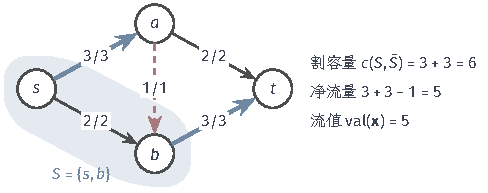
\includegraphics[width=82.564mm]{figures/01-basic-mathematics/04-graphs/tikz/c3-flow-network-cut/figure.pdf}
  \caption{流网络、流与割。弧旁的“$x/c$”表示流量与容量，每个中间顶点流入等于流出，流值为$5$。浅色底标出割的源侧$S=\{s,b\}$：跨出的弧$s\to a$、$b\to t$（蓝色粗弧）的容量计入割容量$3+3=6$；指回的弧$a\to b$（红色虚线）不计容量，其流量在净流量中扣除，$3+3-1=5$。}
  \label{fig:graph-opt-flow-network-cut}
\end{figure}

\subsection{残量网络}
\label{sec:graph-opt-residual-network}

最朴素的改进办法是：找一条从$s$到$t$、每条弧都还有剩余容量的路径，沿它多送一些。但已经选定的路线可能占用了更好的安排，只会追加流量的办法会过早卡住。下面的例子会说明这一点，补救的办法是允许撤回一部分旧流量，把撤回也当作一种可以使用的“通道”。

\paragraph{正向残量与反向残量}
给定流$\bm x$，对每条原弧$u\to v$建立两条\emph{残量弧}：正向残量弧$u\to v$，容量$c_{u,v}-x_{u,v}$，表示还能追加多少；反向残量弧$v\to u$，容量$x_{u,v}$，表示能撤回多少。只保留容量为正的残量弧，得到的有向图称为\term{残量网络}（residual network），记作$\mathcal G_{\bm x}$，残量弧的容量记作$r_{\bm x}$。例如原弧容量为$3$、当前流量为$2$时，正向残量为$1$、反向残量为$2$，如图~\ref{fig:graph-opt-residual-arc}。沿反向残量弧$v\to u$送出一单位，含义是把原弧$u\to v$上的流量减少一单位，并不要求原网络中真有一条从$v$到$u$的管道。

\begin{figure}[!htb]
  \centering
  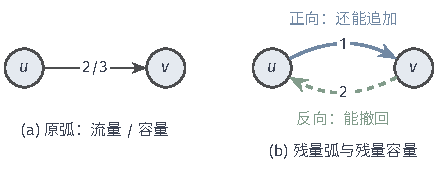
\includegraphics[width=74.186mm]{figures/01-basic-mathematics/04-graphs/tikz/c3-residual-arc/figure.pdf}
  \caption{一条原弧对应两条残量弧。(a) 原弧$u\to v$容量$3$、流量$2$。(b) 残量网络中，正向残量弧$u\to v$（蓝色）容量$3-2=1$，表示还能追加的量；反向残量弧$v\to u$（绿色虚线）容量$2$，表示能撤回的量。流量为$0$时没有反向残量弧，满流时没有正向残量弧。}
  \label{fig:graph-opt-residual-arc}
\end{figure}

\paragraph{撤回旧流的例子}
取弧$s\to a$、$s\to b$、$a\to b$、$a\to t$、$b\to t$，容量都为$1$。若先沿$s\to a\to b\to t$送一单位，三条弧都满了，剩下的$s\to b$与$a\to t$虽有空余，却连不成一条只用正向残量的$s$--$t$路径，只会追加的办法到此停止，流值为$1$。但残量网络中还有反向残量弧$b\to a$，容量$1$，于是出现路径$s\to b\to a\to t$：在$s\to b$与$a\to t$上各追加一单位，同时把$a\to b$上的流量撤回一单位。更新后的流在$s\to a$、$a\to t$、$s\to b$、$b\to t$上各为$1$，在$a\to b$上为$0$，流值为$2$。逐点核对：$a$流入$1$、流出$1$，$b$流入$1$、流出$1$，各弧都不超过容量。图~\ref{fig:graph-opt-undo-flow}画出这三个阶段。最终的实际输送是两条不相交的路线$s\to a\to t$与$s\to b\to t$，第一次选路时经过$a\to b$的那一单位被“改道”了。

\begin{figure*}[!htb]
  \centering
  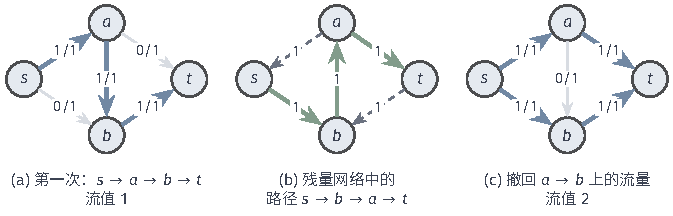
\includegraphics[width=113.901mm]{figures/01-basic-mathematics/04-graphs/tikz/c3-undo-flow/figure.pdf}
  \caption{单位容量网络中撤回旧流量。(a) 先沿$s\to a\to b\to t$送一单位（蓝色粗弧为流量$1$的弧），只用正向残量已无$s$--$t$路径。(b) 残量网络：满流弧只剩反向残量弧（灰色），绿色路径$s\to b\to a\to t$经过反向残量弧$b\to a$。(c) 沿该路径更新后，$a\to b$上的流量被撤回，流值变为$2$，实际路线为$s\to a\to t$与$s\to b\to t$。}
  \label{fig:graph-opt-undo-flow}
\end{figure*}

原网络若同时有$u\to v$与$v\to u$两条弧，残量网络中可能出现两条同向的$u\to v$残量弧：一条是原弧$u\to v$的正向残量，另一条是原弧$v\to u$的反向残量。实现时应保留每条残量弧对应哪条原弧、哪个方向的身份，沿它送流时修改的是对应原弧的流量。否则会把“真实地反向输送”与“撤回另一条弧上的流量”混成同一个量。

\subsection{增广路径与最优性条件}
\label{sec:graph-opt-augmenting-path}

有了残量网络，改进一个流的办法就统一成了找路：残量网络中的任何一条$s$--$t$路径都给出一种在不违反约束的前提下增加流值的调整。

\paragraph{增广路径与瓶颈}
残量网络$\mathcal G_{\bm x}$中从$s$到$t$的简单路径$P$称为关于$\bm x$的\term{增广路径}（augmenting path）。$P$上残量容量的最小值
\[
  \Delta=\min_{(u\to v)\in P}r_{\bm x}(u,v)>0
\]
称为$P$的\term{瓶颈容量}（bottleneck capacity）。沿$P$增广$\Delta$，是指对$P$上的每条残量弧：若它是原弧$u\to v$的正向残量，令$x_{u,v}\leftarrow x_{u,v}+\Delta$；若它是原弧$v\to u$的反向残量，令$x_{v,u}\leftarrow x_{v,u}-\Delta$。

\begin{lemma}[沿增广路径更新保持可行]
\label{lem:graph-opt-augment}
设$\bm x$是流，$P$是增广路径，瓶颈容量为$\Delta$。沿$P$增广$\Delta$后得到的$\bm x'$仍是流，并且$\operatorname{val}(\bm x')=\operatorname{val}(\bm x)+\Delta$。
\end{lemma}

\begin{proof}
容量约束：正向残量弧满足$\Delta\leq c_{u,v}-x_{u,v}$，追加后不超过容量；反向残量弧满足$\Delta\leq x_{v,u}$，撤回后不小于零。流守恒：$P$是简单路径，经过每个中间顶点$v$恰好一次，一条残量弧进入$v$，一条离开$v$。进入的那条若是正向残量，$v$的流入增加$\Delta$；若是反向残量，即撤回一条从$v$出发的原弧上的流量，$v$的流出减少$\Delta$。两种情形都使$v$的净流出减少$\Delta$。同理，离开的那条残量弧使$v$的净流出增加$\Delta$。两者相抵，$v$仍满足守恒。最后，$P$的第一条残量弧离开$s$，使$s$的净流出增加$\Delta$，而$P$是简单路径，不再回到$s$，所以流值增加$\Delta$。
\end{proof}

\paragraph{同值割证书}
引理说明，只要存在增广路径，当前流就不是最大流。反过来，没有增广路径时，能否断定当前流最大？答案是肯定的，而且可以从残量网络中直接读出一个与流值相等的割。

\begin{theorem}[增广路径判据]
\label{thm:graph-opt-augmenting-path}
设$\bm x$是流网络上的一个流，则下列三条等价：
\begin{enumerate}
  \item $\bm x$是最大流；
  \item 残量网络$\mathcal G_{\bm x}$中不存在增广路径；
  \item 存在某个$s$--$t$割$(S,\bar S)$，使$\operatorname{val}(\bm x)=c(S,\bar S)$。
\end{enumerate}
此时$(S,\bar S)$是割容量最小的$s$--$t$割，可取$S$为$\mathcal G_{\bm x}$中从$s$可达的顶点集。
\end{theorem}

\begin{proof}
由1推2：若存在增广路径，由引理~\ref{lem:graph-opt-augment}可得流值更大的流，与$\bm x$最大矛盾。

由2推3：令$S$为$\mathcal G_{\bm x}$中从$s$可达的顶点集。$s\in S$，而没有增广路径说明$t\notin S$，所以$(S,\bar S)$是$s$--$t$割。考察跨割的原弧。若$u\in S$、$v\in\bar S$且$u\to v$是原弧，则必有$x_{u,v}=c_{u,v}$，否则正向残量弧$u\to v$存在，$v$就从$s$可达了。若$v\in\bar S$、$u\in S$且$v\to u$是原弧，则必有$x_{v,u}=0$，否则反向残量弧$u\to v$存在，同样使$v$可达。把这两条代入式~\eqref{eq:graph-opt-net-flow-cut}，第一个和等于$c(S,\bar S)$，第二个和为零，故$\operatorname{val}(\bm x)=c(S,\bar S)$。

由3推1：对任意流$\bm y$，引理~\ref{lem:graph-opt-weak-duality}给出$\operatorname{val}(\bm y)\leq c(S,\bar S)=\operatorname{val}(\bm x)$，所以$\bm x$最大。同一不等式对任意割$(S',\bar S')$给出$c(S',\bar S')\geq\operatorname{val}(\bm x)=c(S,\bar S)$，所以$(S,\bar S)$的割容量最小。
\end{proof}

割容量最小的$s$--$t$割称为\term{最小割}（minimum cut）。定理把“是否最优”这个关于全部候选流的问题，化成了在残量网络中做一次遍历就能回答的问题；停止时得到的流与割互为证书，任何人都可以逐弧核对两者的数值相等，而不必相信算法本身。图~\ref{fig:graph-opt-max-flow-certificate}是第~\ref{sec:graph-opt-flow-cut}小节网络的一个最大流及其证书：残量网络中$s$的两条出弧都已满流，从$s$出发哪里也去不了，$S=\{s\}$，割容量$3+2=5$等于流值。

\begin{figure}[!htb]
  \centering
  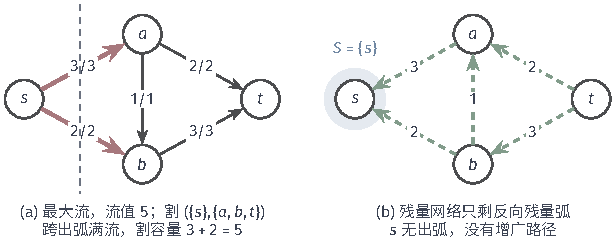
\includegraphics[width=104.186mm]{figures/01-basic-mathematics/04-graphs/tikz/c3-max-flow-certificate/figure.pdf}
  \caption{最大流与最小割互为证书。(a) 原网络上的最大流，弧旁为“流量/容量”，流值为$5$；虚线表示割$(\{s\},\{a,b,t\})$，其跨出弧$s\to a$、$s\to b$（红色）均满流，割容量$3+2=5$等于流值。(b) 对应的残量网络：五条原弧都已满流，只剩反向残量弧（绿色虚线），弧旁为残量容量；$s$没有出弧，从$s$可达的集合为$S=\{s\}$（浅色底），不存在增广路径。}
  \label{fig:graph-opt-max-flow-certificate}
\end{figure}

需要注意定理的范围。它判定一个\emph{给定}的流是否最优，并在最优时给出证书；它没有断言任意选路的增广过程一定会在有限步内走到这样的流，也还没有说明最大流一定存在。存在性由第~\ref{sec:graph-opt-edmonds-karp}小节的Edmonds--Karp算法以构造的方式补齐。

\subsection{Ford--Fulkerson增广法}
\label{sec:graph-opt-ford-fulkerson}

定理~\ref{thm:graph-opt-augmenting-path}直接给出一个算法框架：从零流出发，只要残量网络中还有增广路径就沿它增广，没有时停止。这个框架称为\term{Ford--Fulkerson方法}（Ford--Fulkerson method）。称它为“方法”，是因为它没有规定选哪条增广路径。

\begin{algorithm}[Ford--Fulkerson增广法]
\label{alg:graph-opt-ford-fulkerson}
输入：流网络$(\mathcal G,c,s,t)$。输出：流$\bm x$与割$(S,\bar S)$。状态：各原弧的流量、由流量确定的正反残量、搜索用的前驱与当前流值。
\begin{enumerate}
  \item 令$\bm x=\bm 0$。
  \item 在当前残量网络中搜索一条$s$--$t$路径，记录前驱；若没有，转第4步。
  \item 沿前驱恢复路径$P$，求瓶颈$\Delta$，按引理~\ref{lem:graph-opt-augment}更新对应原弧的流量，流值加$\Delta$，回到第2步。
  \item 令$S$为最后一次搜索中从$s$可达的顶点集，输出$\bm x$与$(S,\bar S)$。
\end{enumerate}
\end{algorithm}

每次更新都会改变若干残量：正向残量减少，反向残量增加，有的残量弧消失，也有新的出现。所以每轮都要在更新后的残量网络中重新搜索，不能沿用上一轮找到的其他路径。

\paragraph{算例}
回到图~\ref{fig:graph-opt-flow-network-cut}的网络，弧$s\to a$、$s\to b$、$a\to b$、$a\to t$、$b\to t$的容量依次为$3,2,1,2,3$。从零流出发：
\begin{enumerate}
  \item 沿$s\to a\to t$增广，瓶颈$\min\{3,2\}=2$，流值为$2$；
  \item 沿$s\to b\to t$增广，瓶颈$\min\{2,3\}=2$，流值为$4$；
  \item 此时$s\to a$剩余$1$，$a\to t$已满，沿$s\to a\to b\to t$增广，瓶颈$\min\{1,1,1\}=1$，流值为$5$。
\end{enumerate}
所得流在五条弧上依次为$3,2,1,2,3$，每条弧都满流。$a$流入$3$、流出$1+2=3$，$b$流入$2+1=3$、流出$3$，守恒成立。残量网络中$s$的两条出弧都已饱和，搜索停止，得到$S=\{s\}$，即图~\ref{fig:graph-opt-max-flow-certificate}中的证书。前面的单位容量例子也是这个框架的一次运行：先选了$s\to a\to b\to t$，第二轮的增广路径$s\to b\to a\to t$经过反向残量弧，撤回了旧的流量。

\paragraph{整数容量下的有限终止}
框架是否总会停止？容量都是整数时，答案是肯定的。

\begin{theorem}[整数容量下的有限终止]
\label{thm:graph-opt-integer-termination}
若所有容量都是非负整数，则Ford--Fulkerson方法无论怎样选择增广路径，至多经过$C_s=\sum_{w:\,s\to w}c_{s,w}$次增广就停止，输出的流是最大流，并且每条弧上的流量都是整数。
\end{theorem}

\begin{proof}
对增广次数归纳可知，流量始终是整数：零流是整数的；若当前流量都是整数，则残量$c_{u,v}-x_{u,v}$与$x_{u,v}$都是整数，瓶颈$\Delta$是正整数，更新后流量仍为整数。于是每次增广使流值至少增加$1$。另一方面，由引理~\ref{lem:graph-opt-weak-duality}，取$S=\{s\}$可知流值不超过$C_s$。所以增广至多$C_s$次。停止时没有增广路径，由定理~\ref{thm:graph-opt-augmenting-path}，所得流最大。
\end{proof}

这个定理同时说明，整数容量的网络存在每条弧流量都为整数的最大流，第~\ref{sec:graph-matching}节的匹配会用到这一点。容量为有理数时，乘以公分母即化为整数情形。但对一般的实容量，上面的整数步长论证不能照搬：每次流值都增加，增加量却可能越来越小。已知存在容量含无理数的网络，任意选路的Ford--Fulkerson方法可以永不停止，流值甚至收敛到小于最大流值的数。因此，任意选路的框架不自动具有有限终止的保证，需要对选路规则加以限制。

\subsection{Edmonds--Karp算法}
\label{sec:graph-opt-edmonds-karp}

Edmonds--Karp算法保留残量网络与增广更新，只对选路加一条规则：每次用广度优先遍历寻找弧数最少的增广路径。这里的“最短”按残量弧的条数计算，容量不参与路径长短的比较。

\begin{algorithm}[Edmonds--Karp算法]
\label{alg:graph-opt-edmonds-karp}
与算法~\ref{alg:graph-opt-ford-fulkerson}相同，只是第2步固定用第~\ref{sec:graph-bfs}节的广度优先遍历在残量网络中从$s$搜索，所得前驱路径是弧数最少的$s$--$t$路径。
\end{algorithm}

\paragraph{算例}
在同一个$3,2,1,2,3$网络上按字母顺序访问邻居，记$h(v)$为$v$在当前残量网络中的广度优先层数，即从$s$出发的最少弧数。第$1$轮，各层为$h(a)=h(b)=1$、$h(t)=2$，选出$s\to a\to t$，瓶颈$2$。第$2$轮，残量网络中$s\to a$剩$1$、$a\to t$已满，层数仍为$h(a)=h(b)=1$、$h(t)=2$，选出$s\to b\to t$，瓶颈$2$。第$3$轮，$s\to b$已满，$b$只能经$a$到达，层数变为$h(a)=1$、$h(b)=2$、$h(t)=3$，选出$s\to a\to b\to t$，瓶颈$1$。第$4$轮从$s$出发不能到达任何顶点，停止，流值为$5$。图~\ref{fig:graph-opt-edmonds-karp-layers}画出各轮的残量网络与分层。

\begin{figure*}[!htb]
  \centering
  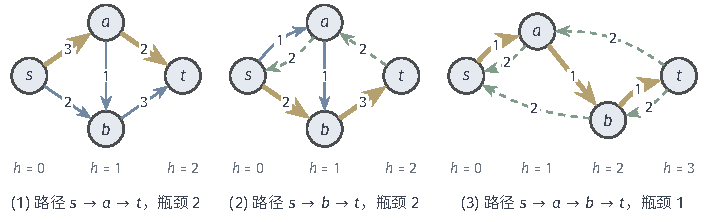
\includegraphics[width=119.567mm]{figures/01-basic-mathematics/04-graphs/tikz/c3-edmonds-karp-layers/figure.pdf}
  \caption{Edmonds--Karp算法在$3,2,1,2,3$网络上的三轮增广。每个面板是该轮开始时的残量网络，顶点按广度优先层数$h$从左到右排列，弧旁为残量容量，蓝色为正向残量弧，绿色虚线为反向残量弧；黄色粗箭头是本轮选出的弧数最少的增广路径。汇点层数依次为$2,2,3$，不随增广而减小。}
  \label{fig:graph-opt-edmonds-karp-layers}
\end{figure*}

这个网络上，Edmonds--Karp算法选出的路径恰好与前面手工选择的相同。差别在单位容量的例子中显现：任意选路时可以先选三条弧的$s\to a\to b\to t$，随后不得不撤回；Edmonds--Karp算法第一轮只会选两条弧的$s\to a\to t$，第二轮选$s\to b\to t$，两次增广即达到流值$2$，不需要撤回。

\paragraph{层数不下降}
增广次数的上界来自层数的变化。记$h_{\bm x}(v)$为$v$在$\mathcal G_{\bm x}$中从$s$出发的最少弧数，不可达时为$+\infty$。首先证明，沿最短增广路径增广不会让任何顶点离$s$更近。

\begin{lemma}[残量层数单调不减]
\label{lem:graph-opt-levels-monotone}
设$\bm x'$由$\bm x$沿$\mathcal G_{\bm x}$中一条弧数最少的增广路径增广得到，则对每个顶点$v$都有$h_{\bm x'}(v)\geq h_{\bm x}(v)$。
\end{lemma}

\begin{proof}
假设结论不成立，在所有满足$h_{\bm x'}(v)<h_{\bm x}(v)$的顶点中取$h_{\bm x'}(v)$最小的一个$v$。显然$v\neq s$。取$\mathcal G_{\bm x'}$中一条$s$到$v$的最短路径，设其最后一条弧为$u\to v$，则$h_{\bm x'}(u)=h_{\bm x'}(v)-1$；由$v$的最小性，$h_{\bm x'}(u)\geq h_{\bm x}(u)$。分两种情形。

若弧$u\to v$在增广前已在$\mathcal G_{\bm x}$中，则$h_{\bm x}(v)\leq h_{\bm x}(u)+1\leq h_{\bm x'}(u)+1=h_{\bm x'}(v)$，与假设矛盾。

若$u\to v$在增广前不在$\mathcal G_{\bm x}$中，它是增广新产生的残量弧。增广只会让路径上残量弧的反向弧获得正容量，所以$v\to u$在增广路径上。增广路径是弧数最少的路径，路径上相邻顶点的层数相差一，故$h_{\bm x}(u)=h_{\bm x}(v)+1$。于是$h_{\bm x}(v)=h_{\bm x}(u)-1\leq h_{\bm x'}(u)-1=h_{\bm x'}(v)-2$，同样矛盾。
\end{proof}

\paragraph{增广次数的上界}
每次增广中，瓶颈弧的残量降为零，从残量网络中消失，称它在这次增广中\emph{饱和}。下面说明同一条残量弧不能频繁地饱和。

\begin{theorem}[Edmonds--Karp算法的增广次数]
\label{thm:graph-opt-edmonds-karp}
在有限实容量的流网络上，Edmonds--Karp算法至多进行$na$次增广就停止。
\end{theorem}

\begin{proof}
残量弧按其对应的原弧与方向区分，至多有$2a$条。固定其中一条$u\to v$。它在某次增广中饱和时位于最短增广路径上，所以$h_{\bm x}(v)=h_{\bm x}(u)+1$，随后从残量网络中消失。它要再次出现，必须在之后的某次增广中，反向弧$v\to u$位于当时的增广路径上，设当时的流为$\bm x''$，则$h_{\bm x''}(u)=h_{\bm x''}(v)+1$。由引理~\ref{lem:graph-opt-levels-monotone}，层数不下降，所以
\[
  h_{\bm x''}(u)=h_{\bm x''}(v)+1\geq h_{\bm x}(v)+1=h_{\bm x}(u)+2.
\]
也就是说，$u\to v$相邻两次饱和之间，$u$的层数至少增加$2$。$u$作为增广路径上的非汇点顶点，其层数在$0$到$n-2$之间，因此$u\to v$至多饱和$n/2$次。每次增广至少饱和一条残量弧，总增广次数不超过$2a\cdot n/2=na$。
\end{proof}

这个界只依赖顶点数与弧数，与容量的数值无关，所以对任意有限实容量都成立。算法停止时没有增广路径，由定理~\ref{thm:graph-opt-augmenting-path}，所得流最大，残量可达集给出最小割。这就以构造的方式证明了最大流的存在，并得到本节的核心结论。

\begin{theorem}[最大流最小割定理]
\label{thm:graph-opt-max-flow-min-cut}
在有限非负实容量的流网络中，最大流存在，并且最大流值等于最小$s$--$t$割的割容量。
\end{theorem}

\begin{proof}
由定理~\ref{thm:graph-opt-edmonds-karp}，Edmonds--Karp算法有限步停止，输出流$\bm x$在残量网络中没有增广路径。由定理~\ref{thm:graph-opt-augmenting-path}，$\bm x$是最大流，且存在割$(S,\bar S)$使$\operatorname{val}(\bm x)=c(S,\bar S)$，这个割的割容量最小。
\end{proof}

这一结论通常称为\term{最大流最小割定理}（max-flow min-cut theorem）。容量都是整数时，Edmonds--Karp算法作为Ford--Fulkerson方法的特例，每次更新仍保持整数流，所以它输出的最大流是整数流。

\subsection{算法分析与结果检验}
\label{sec:graph-opt-max-flow-analysis}

两种算法的增广次数界依据不同，应当分开陈述。Ford--Fulkerson方法在整数容量下的界$C_s$依赖容量的数值：容量放大一千倍，界也放大一千倍，它不是输入位长的多项式。Edmonds--Karp算法的界$na$只依赖网络的规模。任意选路的版本不能借用后者。

\paragraph{运行时间}
先在线性时间内删去既非源汇、又不与任何弧关联的孤立点，它们不影响流，删去后$n\leq2a+2$，于是$O(n+a)=O(a)$。Edmonds--Karp算法每轮在残量网络中做一次广度优先遍历，扫描至多$2a$条残量弧，再沿路径更新流量，用时$O(a)$。乘以$O(na)$轮，总时间为$O(na^2)$次算术与比较操作。这是在每次加减比较都算一步的模型下的计数，不是不加条件的位复杂度结论。Ford--Fulkerson方法在整数容量下每轮搜索同样是$O(n+a)$，总时间为$O(C_s(n+a))$。

\paragraph{结果检验}
算法应输出原网络上的流$\bm x$、残量可达集确定的割$(S,\bar S)$以及共同的数值。检验时逐项核对：每条弧满足$0\leq x_{u,v}\leq c_{u,v}$；每个中间顶点流入等于流出；源点净流出与汇点净流入相等；割容量按跨出弧重新求和，并与流值比较。两者相等时，由引理~\ref{lem:graph-opt-weak-duality}，流与割同时最优，检验不依赖算法过程本身。在本节的算例中，流值为$5$，割$\{s\}$的容量也是$5$。

最小割不一定唯一。在同一网络中，$S=\{s,a\}$的跨出弧为$s\to b$、$a\to b$、$a\to t$，容量$2+1+2=5$；$S=\{s,a,b\}$的跨出弧为$a\to t$、$b\to t$，容量$2+3=5$；只有$S=\{s,b\}$的容量为$6$。三个最小割都能与流值$5$构成证书，残量可达集给出的是其中源侧最小的一个。

若计算采用浮点数，守恒、容量与同值比较都只能在误差范围内成立，应分别报告守恒误差、容量违反量以及流值与割容量之差，而不能把近似满足直接称为精确证书。

\paragraph{后续用途}
最大流与最小割会在后面多次出现，但每次都要先说明问题怎样转成当前的网络与目标。第~\ref{sec:graph-min-cost-flow}节固定各点的供需量，转而比较输送费用；第~\ref{sec:graph-matching}节用单位容量的网络把二部图匹配写成整数流；第~\ref{sec:graph-pairwise-binary-cut}节把一类二值变量的成对目标写成割容量，再用最小割求解。仅凭这些问题都画在图上，并不能共享最优性结论，模型的转换关系必须逐一建立。

% 第3章第4节：最小费用流（问题与下界平移；负费用环判据、节点势与逐弧证书；网络单纯形法；算法分析与结果检验）。

\section{最小费用流}
\label{sec:graph-min-cost-flow}

第~\ref{sec:graph-max-flow}节只问能送多少：源点送出得越多越好，货物走哪条路、花多少代价并不计较。实际调运中，各处的产量与需求往往事先给定，同一批货物可以经由不同线路到达，而各条线路的单位运价不同。这时要比较的不再是输送量，而是在满足固定供需的全部方案中，哪一个总费用最低。

本节先写出带供需、上下界和单位费用的最小费用流问题，并把一般下界化成零下界。随后建立最优性条件：一个可行流最优，当且仅当它的残量网络中没有负费用环；引入节点势后，这一条件可以逐弧检查。在此基础上介绍\term{网络单纯形法}（network simplex method，亦称网络单形法）。它把可行流组织在一棵生成树上，沿树上的环逐步降低费用，停止时同时给出由流量与节点势组成的最优性证书。网络单纯形法是线性规划单纯形法在网络上的特例，一般单纯形法的系统理论留到后续优化部分；这里只用树、环和守恒式直接建立它的各个步骤。后面的匹配与指派两节各有专门的增广算法，阅读它们不以掌握本节的全部换基细节为前提。

\subsection{最小费用流问题}
\label{sec:graph-opt-mcf-problem}

设想几个仓库向几家商店供货。仓库的库存要全部运出，商店的需求要恰好满足，中转站既不生产也不消耗；每条运输线路有运量上限，有些线路按合同还有最低运量，每运一单位货物要付相应的运价。把仓库、商店和中转站看成顶点，线路看成有向弧，就得到下面的问题。为了把字母$c$留给费用，本节把第~\ref{sec:graph-max-flow}节的容量改记为上界$u_{i,j}$，弧写作$(i,j)$或$i\to j$。

\begin{definition}[最小费用流问题]
\label{def:graph-opt-min-cost-flow}
设$\mathcal G=(V,E)$是有限有向图，每个顶点$i$有供需量$b_i\in\mathbb R$，每条弧$(i,j)\in E$有有限的下界$\ell_{i,j}$、上界$u_{i,j}$（$\ell_{i,j}\leq u_{i,j}$）与单位费用$c_{i,j}\in\mathbb R$。给每条弧赋一个流量$x_{i,j}$，若向量$\bm x$满足
\begin{equation}
\begin{gathered}
  \sum_{j:\,(i,j)\in E}x_{i,j}-\sum_{j:\,(j,i)\in E}x_{j,i}=b_i\quad(i\in V),\\
  \ell_{i,j}\leq x_{i,j}\leq u_{i,j}\quad((i,j)\in E),
\end{gathered}
  \label{eq:graph-opt-mcf-constraints}
\end{equation}
则称$\bm x$为可行流。\term{最小费用流}（minimum-cost flow）问题是在全部可行流中最小化总费用$\sum_{(i,j)\in E}c_{i,j}x_{i,j}$。
\end{definition}

守恒式左边是顶点$i$的净流出，所以$b_i>0$表示$i$是供给点，要净送出$b_i$单位；$b_i<0$表示需求点，要净收进$-b_i$单位；$b_i=0$的顶点只做中转。与最大流相比，这里没有单独的源点和汇点：每个顶点的净流出都已事先指定，流值不再是待优化的量，被比较的只有费用。最大流中的守恒式对应中间顶点$b_i=0$，容量约束对应$\ell_{i,j}=0$。

把全部守恒式相加，每条弧的流量在起点计一次正、在终点计一次负，左边相消为零，所以可行流存在的必要条件是$\sum_{i\in V}b_i=0$。这个条件并不充分：总供给等于总需求，不保证货物有路可走，也不保证线路容量够用。图~\ref{fig:graph-opt-mcf-network}的网络中，$s$供给$3$单位、$t$需求$3$单位；若把$s\to a$与$s\to t$的容量都改成$1$，从$s$出发的总容量只有$2$，供需虽然平衡，问题却没有可行流。

\begin{figure}[!htb]
  \centering
  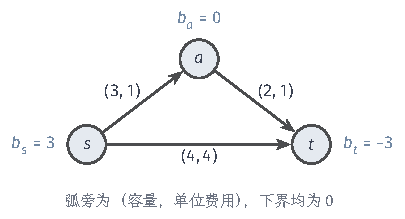
\includegraphics[width=68.527mm]{figures/01-basic-mathematics/04-graphs/tikz/c3-mcf-network/figure.pdf}
  \caption{三点最小费用流算例。$s$供给$3$单位，$t$需求$3$单位，$a$只做中转；弧旁括号依次为容量与单位费用，下界均为$0$。绕行$s\to a\to t$的单位费用为$2$，低于直达弧的$4$，但绕行量受$a\to t$的容量$2$限制。本节后面的计算都在这个网络上进行。}
  \label{fig:graph-opt-mcf-network}
\end{figure}

这个网络有许多可行流。$3$单位全走直达弧，费用为$3\times4=12$；让$2$单位绕行、$1$单位直达，费用为$2\times(1+1)+1\times4=8$。按弧序$s\to a$、$a\to t$、$s\to t$把流量写成向量，前者为$(0,0,3)$，后者为$(2,2,1)$。后面将证明$8$就是最小费用。

\paragraph{下界平移}
带正下界的弧在建模中很常见，例如合同规定某条线路至少运多少。处理办法是先把下界部分“预先送出”，再对剩余部分求解。令$x_{i,j}=\ell_{i,j}+y_{i,j}$，新变量满足$0\leq y_{i,j}\leq u_{i,j}-\ell_{i,j}$。预先送出的下界流量已经使顶点$i$净流出$\sum_j\ell_{i,j}-\sum_j\ell_{j,i}$，代入守恒式，$\bm y$应满足的剩余供需为
\[
  b'_i=b_i-\sum_{j:\,(i,j)\in E}\ell_{i,j}+\sum_{j:\,(j,i)\in E}\ell_{j,i}.
\]
目标变为$\sum c_{i,j}y_{i,j}+\bm c^{\top}\bm\ell$，后一项与$\bm y$无关。两个问题的可行解通过$\bm x=\bm\ell+\bm y$一一对应，费用处处相差同一个常数，所以最优解也一一对应。

图~\ref{fig:graph-opt-mcf-lower-bound}把三点网络中$s\to t$的下界改为$1$。平移后这条弧的容量从$4$变为$3$，同时$s$的剩余供给从$3$降为$2$，$t$的剩余需求从$3$降为$2$。如果只把容量减去下界而不修改供需，平移后的问题仍要求$s$送出$3$单位，下界那一单位就被重复计算了。新问题的最优解是$\bm y=(2,2,0)$，费用为$4$；加回常数$c_{s,t}\ell_{s,t}=4$，得到原问题的最优流$\bm x=(2,2,1)$与费用$8$。

\begin{figure}[!htb]
  \centering
  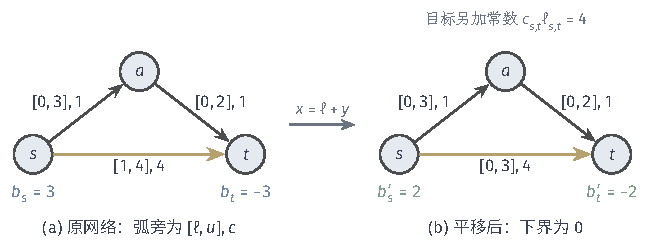
\includegraphics[width=109.767mm]{figures/01-basic-mathematics/04-graphs/tikz/c3-mcf-lower-bound-shift/figure.pdf}
  \caption{下界平移。(a)中黄色弧$s\to t$的流量须在$[1,4]$内，弧旁依次为流量区间与单位费用。(b)令$x=\ell+y$后，该弧的区间变为$[0,3]$，$s$与$t$的供需同时各减少$1$单位（绿色），目标另加常数$4$。容量和供需必须一起修改，只改其一会重复或遗漏下界那一单位。}
  \label{fig:graph-opt-mcf-lower-bound}
\end{figure}

上下界相等的弧流量已经固定，平移后容量为零，可以先删去，只保留它对供需和常数的贡献。还原时把平移量加回流量、把常数加回费用即可。以下除非特别说明，都假定下界已平移为零，固定弧已删去。

\paragraph{最优解的存在}
在有限上下界下，可行流集合由有限个线性等式与闭区间约束确定，是$\mathbb R^{a}$中的闭有界集，其中$a=|E|$。总费用是$\bm x$的线性函数，因而连续。由闭有界集上的极值定理~\ref{thm:multivariable-extreme-value}，只要可行流存在，最小费用一定能取到。可行流是否存在要另外判断，后文网络单纯形法的第一阶段就承担这一任务。

若允许某些弧的容量为无穷，可行集不再有界，最小值可能不存在。设可行流$\bm x$的残量网络（下一小节定义）中有一个负费用环，环上每条残量弧的剩余容量都是无穷，那么沿这个环可以推送任意多的流量，每推一单位都减少同样的正费用，总费用没有下界。本节主线只讨论有限容量。

还有一类常见问题：在源汇网络中先尽量多送，再在全部最大流中挑费用最低的，称为最小费用最大流。它分两步化成本节的问题：先用第~\ref{sec:graph-max-flow}节的方法求出最大流值$v^\star$，再令$b_s=v^\star$、$b_t=-v^\star$、其余$b_i=0$，求最小费用流。

\subsection{最优性条件}
\label{sec:graph-opt-mcf-optimality}

拿到一个可行流后，怎样判断它是否已经最便宜？逐一比较全部可行流行不通。第~\ref{sec:graph-max-flow}节判断最大流时，用残量网络把问题化成了“能否找到一条增广路径”。本小节沿用这一思路：先用残量网络描述所有保持供需的调整，再说明费用能否下降取决于其中是否有负费用环，最后借助节点势把环条件改写成逐弧可查的不等式。

\paragraph{残量网络与负费用环}
给定可行流$\bm x$。对每条原弧$(i,j)$，若$x_{i,j}<u_{i,j}$，建立正向残量弧$i\to j$，剩余容量为$u_{i,j}-x_{i,j}$，费用为$c_{i,j}$，表示再追加一单位要多付$c_{i,j}$；若$x_{i,j}>\ell_{i,j}$，建立反向残量弧$j\to i$，剩余容量为$x_{i,j}-\ell_{i,j}$，费用为$-c_{i,j}$，表示撤回一单位可以省下$c_{i,j}$。这与第~\ref{sec:graph-max-flow}节的残量网络相同，只是每条残量弧多带一个费用。原网络同时有$i\to j$与$j\to i$两条弧时，各自的残量弧要记住来自哪条原弧，不能合并成一个量。

沿残量网络中的有向环$C$推送$\theta>0$单位，是指对环上每条残量弧调整它的来源原弧：正向残量弧对应的原弧流量加$\theta$，反向残量弧对应的原弧流量减$\theta$。环上每个顶点恰有一条环弧进入、一条环弧离开，调整前后它的净流出不变，所以供需仍然满足；只要$\theta$不超过环上的最小剩余容量，上下界也仍然满足。总费用的改变量是$\theta\,c(C)$，其中$c(C)$是环上残量费用之和。于是，若$c(C)<0$，取正步长就能严格降低费用，当前流不是最优。

图~\ref{fig:graph-opt-mcf-residual-cycle}从全部走直达弧的可行流出发。残量网络中，$s\to a$与$a\to t$两条正向残量弧各费$1$，直达弧的反向残量弧$t\to s$费$-4$，三者构成费用为$1+1-4=-2$的环，剩余容量为$\min\{3,2,3\}=2$。沿这个环推送$2$单位，相当于把$2$单位从直达改为绕行，费用从$12$降为$12-2\times2=8$。

\begin{figure}[!htb]
  \centering
  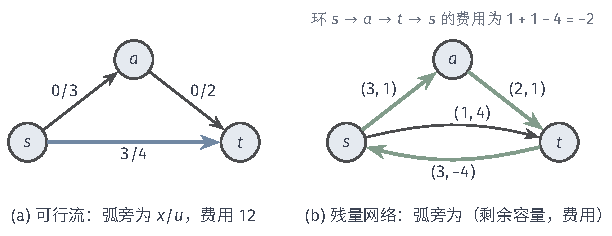
\includegraphics[width=103.579mm]{figures/01-basic-mathematics/04-graphs/tikz/c3-mcf-residual-cycle/figure.pdf}
  \caption{残量网络中的负费用环。(a)全部$3$单位走直达弧的可行流，弧旁为流量与容量。(b)它的残量网络，弧旁为剩余容量与费用；直达弧同时产生可追加$1$单位的正向残量弧和可撤回$3$单位、费用$-4$的反向残量弧$t\to s$。绿色环的费用为$-2$，沿它推送$2$单位使总费用降低$4$。}
  \label{fig:graph-opt-mcf-residual-cycle}
\end{figure}

\paragraph{环分解与最优性判据}
负费用环使费用可以下降。反过来，若残量网络中没有负费用环，是否就不存在更便宜的可行流？为此要说明：任何一个可行流与当前流之差，都能拆成残量网络中若干个环的叠加。

\begin{theorem}[负费用环判据]
\label{thm:graph-opt-negative-cycle}
可行流$\bm x$是最小费用流，当且仅当它的残量网络中不存在费用为负的有向环。
\end{theorem}

\begin{proof}
必要性已由上面的推送论证给出，下证充分性。任取可行流$\bm x'$，令$\bm d=\bm x'-\bm x$。两个流满足同一组供需，所以$\bm d$在每个顶点的净流出为零。逐条考察原弧$(i,j)$：若$d_{i,j}>0$，则$x_{i,j}<x'_{i,j}\leq u_{i,j}$，正向残量弧存在且剩余容量至少为$d_{i,j}$，在它上面放$d_{i,j}$；若$d_{i,j}<0$，则$x_{i,j}>x'_{i,j}\geq\ell_{i,j}$，反向残量弧存在，在它上面放$-d_{i,j}$。这样得到残量弧上的一组非负数$\bm g$，它在每个顶点的流入等于流出，并且按残量费用加权的总和等于$\sum_{(i,j)}c_{i,j}d_{i,j}=\bm c^{\top}\bm x'-\bm c^{\top}\bm x$。

接着把$\bm g$拆成环。若$\bm g\neq\bm 0$，从任一取正值的残量弧出发，沿正值弧前进：每到达一个顶点，它的流入为正，由流入等于流出，必有一条正值出弧可走。顶点只有有限个，前进中必然首次回到某个走过的顶点，由此截出一个有向环$C_1$。令$\lambda_1>0$为$\bm g$在$C_1$上的最小值，从环上各弧减去$\lambda_1$，剩余部分仍然非负且守恒，而取正值的弧至少少了一条。重复有限次，得到
\[
  \bm c^{\top}\bm x'-\bm c^{\top}\bm x=\sum_k\lambda_k\,c(C_k),\qquad\lambda_k>0.
\]
每个$C_k$都由残量弧组成。残量网络中没有负费用环时，右边每项非负，$\bm x'$不比$\bm x$便宜。
\end{proof}

判据回答的是怎样识别最优流，并不断言最优流唯一：若残量网络中有费用为零的环，沿它推送就得到另一个同费用的最优流。判据本身也不是完整的算法。反复寻找负费用环并沿它推送是一种自然的想法，但找哪个环、推多少、何时停止都要另行规定；下面的网络单纯形法给出一种具体的组织方式。

\paragraph{节点势与约化费用}
环判据要求检查所有的环，环的个数可能随图的规模指数增长。为了把它变成逐弧检查，给每个顶点$i$配一个实数$\pi_i$，称为\term{节点势}（node potential），并定义弧$(i,j)$的\term{约化费用}（reduced cost）
\begin{equation}
  \bar c_{i,j}=c_{i,j}-\pi_i+\pi_j.
  \label{eq:graph-opt-reduced-cost}
\end{equation}
残量弧使用同一公式：反向残量弧$j\to i$的费用为$-c_{i,j}$，约化费用为$-c_{i,j}-\pi_j+\pi_i=-\bar c_{i,j}$。

沿任一有向环把约化费用相加，每个顶点的势在离开它的弧上以$-\pi$出现一次、在进入它的弧上以$+\pi$出现一次，两两相消，所以环的约化费用之和等于原费用之和。因此，若能找到一组势，使所有残量弧的约化费用都非负，残量网络就没有负费用环。

反过来，残量网络没有负费用环时，这样的势一定存在。加入一个虚拟顶点$r$，从$r$向每个顶点连一条费用为零的弧。新弧都从$r$出发，没有弧进入$r$，所以新图的环都不经过$r$，仍然没有负环。由第~\ref{sec:graph-shortest-paths}节允许负边长的最短路结论，$r$到每个顶点$i$的最短距离$d_i$都是有限值（且$d_i\leq0$），并且对每条残量弧$i\to j$及其费用$c'$满足距离不等式$d_j\leq d_i+c'$。取$\pi_i=-d_i$，即得
\[
  c'-\pi_i+\pi_j=c'+d_i-d_j\geq0.
\]
所以“残量网络没有负费用环”与“存在使全部残量弧约化费用非负的势”等价，而后者只需逐弧检查。实际计算时可以用Bellman--Ford算法求$d_i$；若算法报告负环，就得到一个可以推送的负费用环。

\paragraph{逐弧最优性证书}
残量弧是否存在取决于原弧流量的位置，所以“全部残量弧的约化费用非负”可以翻译成原弧上的条件。弧$(i,j)$在下界时只有正向残量弧，要求$\bar c_{i,j}\geq0$；在上界时只有反向残量弧，要求$-\bar c_{i,j}\geq0$，即$\bar c_{i,j}\leq0$；严格位于两界之间时两条残量弧都存在，要求$\bar c_{i,j}=0$。下面的定理直接验证这组条件足以保证最优，不必再经过环分解。

\begin{theorem}[节点势最优性证书]
\label{thm:graph-opt-potential-certificate}
设固定弧已删去，$\bm x$是可行流，$\bm\pi$是一组节点势。若对每条弧$(i,j)$都有
\begin{equation}
  \bar c_{i,j}\ \begin{cases}
    \geq0, & x_{i,j}=\ell_{i,j},\\
    \leq0, & x_{i,j}=u_{i,j},\\
    =0, & \ell_{i,j}<x_{i,j}<u_{i,j},
  \end{cases}
  \label{eq:graph-opt-mcf-certificate}
\end{equation}
则$\bm x$是最小费用流。
\end{theorem}

\begin{proof}
任取可行流$\bm x'$。把$c_{i,j}=\bar c_{i,j}+\pi_i-\pi_j$代入费用差，
\[
  \bm c^{\top}(\bm x'-\bm x)=\sum_{(i,j)\in E}\bar c_{i,j}(x'_{i,j}-x_{i,j})+\sum_{(i,j)\in E}(\pi_i-\pi_j)(x'_{i,j}-x_{i,j}).
\]
第二个和按顶点重新归组，等于对每个$i$把$\pi_i$乘以顶点$i$在$\bm x'$与$\bm x$下净流出之差再求和；两个流满足同一组供需，这些差全为零。第一个和逐项非负：若$x_{i,j}=\ell_{i,j}$，则$x'_{i,j}-x_{i,j}\geq0$且$\bar c_{i,j}\geq0$；若$x_{i,j}=u_{i,j}$，则$x'_{i,j}-x_{i,j}\leq0$且$\bar c_{i,j}\leq0$；其余情形$\bar c_{i,j}=0$。所以$\bm c^{\top}\bm x'\geq\bm c^{\top}\bm x$。
\end{proof}

删去固定弧是为了避免$\ell_{i,j}=u_{i,j}$时前两个条件同时出现。条件~\eqref{eq:graph-opt-mcf-certificate}在线性规划中称为互补松弛条件，这里只用守恒式和每条弧允许的变化方向就完成了证明。流量$\bm x$与势$\bm\pi$合在一起构成一份证书：检查者核对可行性和每条弧上的一个符号，就能确认最优性，不必相信求解过程。回到三点网络，流$(2,2,1)$配上势$(\pi_s,\pi_a,\pi_t)=(4,3,0)$时，$s\to a$与$s\to t$都在两界之间，约化费用分别为$1-4+3=0$与$4-4+0=0$；$a\to t$在上界，约化费用为$1-3+0=-2\leq0$。三条弧都满足条件，所以费用$8$最小。

\subsection{网络单纯形法}
\label{sec:graph-opt-network-simplex}

定理~\ref{thm:graph-opt-potential-certificate}说明了停止时应该看到什么：一个可行流和一组势，逐弧满足符号条件。网络单纯形法始终保持流可行，并用一棵生成树确定势：树弧的约化费用被要求为零，由此解出势；再检查非树弧，若全部满足证书就停止，否则沿一个环改进流量。本小节以可行树基为算法状态，依次说明它的表示、第一个可行树基的构造、势的计算、环上的调整与状态更新，以及防止循环的选弧规则，最后用三点网络完整演示。

\paragraph{树基表示}
设下界已平移为零、固定弧已删去，并暂设底层无向图连通，即忽略弧的方向后连通。把弧集分成三部分：树弧集$T$，忽略方向后构成一棵生成树；取下界的非树弧集$L$；取上界的非树弧集$U$。三元组$(T,L,U)$称为一个\term{树基}（spanning tree basis）。非树弧的流量由它所在的集合直接给出，树弧的流量由守恒式决定。生成树总有叶子，叶子$v$只关联一条树弧，$v$的守恒式中其余各项（$b_v$与非树弧流量）都已知，于是解出这条树弧的流量；删去这个叶子及其树弧，把求出的流量计入相邻顶点的剩余供需，再对剩下的树重复，直到树弧全部求出。若求得的树弧流量都在上下界内，就称$(T,L,U)$为可行树基。

这里有两点容易误解。第一，树弧的流量允许恰好等于上界或下界；一条弧是否属于$T$取决于它在树中的位置，而不是流量是否严格在界内。第二，树不要求所有弧都朝向某个根，弧的方向只决定它在守恒式中取正号还是负号。

图~\ref{fig:graph-opt-ns-tree-basis}(a)是一个五点例子，供需为$b=(4,0,-2,1,-3)$，非树弧$1\to4$在上界、流量为$2$，$2\to5$在下界、流量为$0$。叶子$1$的守恒式为$x_{1,2}+x_{1,4}=4$，得$x_{1,2}=2$；叶子$4$的守恒式为$x_{4,3}-x_{1,4}=1$，得$x_{4,3}=3$，恰好等于这条树弧的容量；叶子$5$的守恒式为$-(x_{3,5}+x_{2,5})=-3$，得$x_{3,5}=3$。删去这三个叶子后，顶点$2$成为叶子，由$x_{2,3}+x_{2,5}-x_{1,2}=0$得$x_{2,3}=2$。最后剩下的顶点$3$的守恒式$x_{3,5}-x_{2,3}-x_{4,3}=3-2-3=-2$自动成立，因为全部供需之和为零。

\begin{figure*}[!htb]
  \centering
  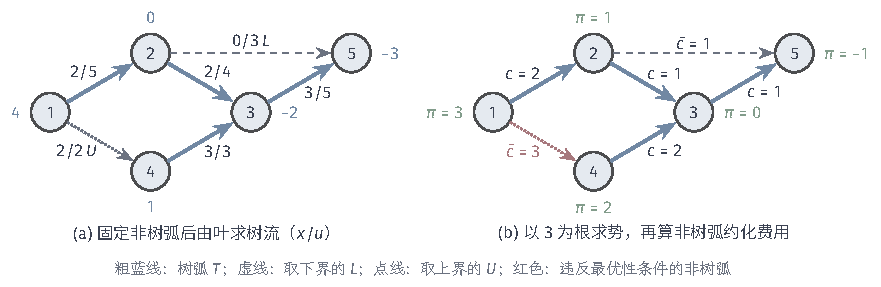
\includegraphics[width=149.144mm]{figures/01-basic-mathematics/04-graphs/tikz/c3-ns-tree-basis/figure.pdf}
  \caption{五点网络上的树基。粗蓝弧为树弧，虚线弧取下界，点线弧取上界。(a)顶点旁为供需量，弧旁为流量与容量；固定两条非树弧后，从叶子$1,4,5$开始逐个用守恒式求出树弧流量，树弧$4\to3$恰在上界仍属于树。(b)弧旁为单位费用或约化费用，绿色为以顶点$3$为根求出的节点势；树弧约化费用均为零，非树弧$1\to4$在上界却有$\bar c=3>0$（红色），违反最优性条件。}
  \label{fig:graph-opt-ns-tree-basis}
\end{figure*}

树流为什么由树唯一确定，可以用关联矩阵说明。按第~\ref{sec:graph-representations}节的约定，关联矩阵$\bm B\in\mathbb R^{n\times a}$中弧$(i,j)$对应的列在第$i$行为$1$、第$j$行为$-1$，守恒式就是$\bm B\bm x=\bm b$。$\bm B$各行之和为零，删去根所在的一行不丢失信息，记剩下的矩阵为$\tilde{\bm B}$。树弧对应的列组成$(n-1)$阶方阵$\tilde{\bm B}_T$。按上面消去叶子的次序排列行与列，每消去一个叶子，它所在的行在剩余树弧列中只有一个非零元，所以$\tilde{\bm B}_T$经行列重排后是三角矩阵，对角元为$\pm1$，从而可逆。于是$\bm x_T=\tilde{\bm B}_T^{-1}(\tilde{\bm b}-\tilde{\bm B}_N\bm x_N)$唯一确定，其中$N=L\cup U$；供需与界都是整数时，树流也是整数。

底层无向图不连通时，在消去固定弧后的各弱连通分量中分别处理：每个分量内的剩余供需之和必须为零，否则问题不可行；孤立顶点没有任何弧，它的供需必须为零。另外，同一个流量可能对应不同的树基，例如树弧恰在界上时，它也可能作为非树弧出现在另一个树基中。后面的退化现象正来自这种区别。

\paragraph{初始可行树基}
任意选一棵生成树、令非树弧取下界，求得的树流未必满足上下界。例如在三点网络中取$T=\{s\to a,a\to t\}$、$s\to t$取下界，叶子$a$与$t$迫使$x_{a,t}=3$，超过容量$2$。因此第一个可行树基要专门构造。

在下界已平移为零的网络中，先令全部原弧流量为零，再增加一个人工根$r$：每个$b_i>0$的顶点连人工弧$i\to r$，流量为$b_i$；每个$b_i<0$的顶点连人工弧$r\to i$，流量为$-b_i$；$b_i=0$的顶点连人工弧$i\to r$，流量为零。人工弧的容量取总供给$\sum_{b_i>0}b_i$，足以容纳这些流量。人工弧构成以$r$为中心的星形生成树，每个原顶点的守恒式都由它唯一的人工弧满足，于是得到一个显式的可行树基。

第一阶段令原弧费用为零、人工弧单位费用为一，目标就是人工流的总量，用下面介绍的同一套入弧、环调整与防循环操作求解。若第一阶段最优值为零，人工弧全部空载，原弧上的流量满足原问题的全部约束；若最优值为正，原问题没有可行流，因为原问题的任何可行流配上全零人工流都会使第一阶段目标为零。这一判定不依赖人为选定的“很大的费用常数”。

第一阶段结束后，删去人工根和全部人工弧。原来的树弧中去掉人工弧，留下一个森林；在原图的每个弱连通分量内，用连接不同森林分量的原非树弧把它补成生成树。补入的弧保持原流量不变，它们本来就在上界或下界，作为树弧恰在界上是允许的。随后恢复原费用、重新计算节点势，并从所得的可行树基重新设置防循环所需的数据，进入第二阶段。

\paragraph{节点势的计算}
给定树基，令根的势为零，沿树逐条解方程$c_{i,j}-\pi_i+\pi_j=0$，使每条树弧的约化费用为零。沿树弧方向从已知的$\pi_i$走到$j$时取$\pi_j=\pi_i-c_{i,j}$，逆着树弧方向从已知的$\pi_j$走到$i$时取$\pi_i=\pi_j+c_{i,j}$。换一个根只让全部势同加一个常数，约化费用不变。树流由供需与非树弧的界状态决定，势则只由树的结构与费用决定，两者分别计算。

图~\ref{fig:graph-opt-ns-tree-basis}(b)以顶点$3$为根：逆着$2\to3$得$\pi_2=0+1=1$，再逆着$1\to2$得$\pi_1=1+2=3$；逆着$4\to3$得$\pi_4=0+2=2$；顺着$3\to5$得$\pi_5=0-1=-1$。随后计算非树弧的约化费用：$2\to5$为$3-1+(-1)=1\geq0$，在下界，符合条件；$1\to4$为$4-3+2=3>0$，却在上界，违反条件。

树弧的约化费用都是零，无论流量位于何处都满足条件~\eqref{eq:graph-opt-mcf-certificate}。所以只要全部非树弧也满足条件，即$L$中的弧$\bar c\geq0$、$U$中的弧$\bar c\leq0$，当前流与势就构成最优性证书，算法停止。寻找违反条件的非树弧，称为定价。

\paragraph{入弧与环调整}
违反条件的非树弧有两类：$L$中$\bar c_{i,j}<0$的弧，应沿正向增加流量；$U$中$\bar c_{i,j}>0$的弧，应沿反向减少流量。选定这样一条入弧后，它与树上连接两端点的唯一路径构成一个环，称为\term{基本环}（fundamental cycle）。按入弧的调整方向给环定向：环上顺着定向经过的弧增加流量，逆着定向经过的弧减少流量。环上每个顶点一进一出，调整保持守恒。

推送一单位时，费用变化是环上各弧费用按增减取正负号之和。把每个$c$换成$\bar c+\pi_i-\pi_j$，势沿环相消，而树弧的约化费用为零，所以单位费用变化恰为入弧在调整方向上的约化费用：正向进入时为$\bar c_{i,j}<0$，反向进入时为$-\bar c_{i,j}<0$。

接着确定能推多远。对环上增加流量的弧计算$u-x$，对减少流量的弧计算$x-\ell$，入弧自身也参加比较，取最小值作为步长$\theta$。按$\theta$沿环更新后守恒仍然成立，上下界也都满足。$\theta>0$时费用严格下降$\theta|\bar c_{i,j}|$；$\theta=0$时流量不变，这种情形留到后面专门讨论。

\paragraph{出弧与状态更新}
达到步长$\theta$的弧称为阻塞弧，可能不止一条，按后述防循环规则从中选出一条。若选中的是树弧，它离开树，按它到达的是下界还是上界归入$L$或$U$，入弧则加入$T$。被删去的弧位于基本环上，删去后树仍然连通且无环，新的$T$仍是生成树。势需要更新：最简单的做法是沿新树从根重新计算一遍，便于逐步复核。更省的做法只调整一部分顶点：删去出弧后树分成两块，只有不含根的那一块的势改变，且同加或同减入弧的约化费用。

若选中的是入弧自身，说明它先到达了另一端的界，便从$L$转入$U$或从$U$转入$L$，树和势都不变。这种\emph{界翻转}同样是合法的一次迭代，所以不能把每一轮都描述为两条不同的弧互相交换。

\begin{algorithm}[网络单纯形法]
\label{alg:graph-opt-network-simplex}
输入：有限有向网络，供需$b_i$，有限上下界与单位费用。输出：最优流$\bm x$、费用与节点势$\bm\pi$，或“不可行”的结论。状态：树基$(T,L,U)$、各弧流量（含扰动系数）、树的父顶点与深度、节点势。
\begin{enumerate}
  \item 平移下界、删去固定弧；在每个弱连通分量内检查供需之和为零。
  \item 第一阶段：增加人工根与人工弧，取星形可行树基，原弧费用为零、人工弧费用为一，并按当前树基设置防循环数据。
  \item 计算节点势与非树弧的约化费用；若没有违反条件的非树弧，转第6步。
  \item 选一条违反条件的入弧，构造基本环，比较环上各弧（含入弧）的剩余量得到步长$\theta$，按防循环规则选出阻塞弧。
  \item 沿环更新流量；若出弧是树弧，作树弧交换，否则作界翻转。回到第3步。
  \item 第一阶段停止时，若人工流总量为正，报告不可行；否则删去人工结构，补成原网络的可行树基，恢复原费用并重新设置防循环数据，以第二阶段身份回到第3步。第二阶段停止时，还原下界平移，返回流量、费用与节点势。
\end{enumerate}
\end{algorithm}

\paragraph{退化与防循环}
步长为零的迭代称为\term{退化换基}（degenerate pivot）。它发生在基本环上某条弧已经处在阻塞方向的界上时，通常就是恰在界上的树弧。图~\ref{fig:graph-opt-ns-degenerate}把三点网络中$s\to t$的容量改为$1$，从$T=\{s\to a,a\to t\}$、$U=\{s\to t\}$出发，流量为$(2,2,1)$，树弧$a\to t$已在上界。势为$(2,1,0)$，$s\to t$在上界而$\bar c_{s,t}=4-2+0=2>0$，应反向进入；基本环上$a\to t$要增加流量，剩余量为$0$，所以$\theta=0$。$a\to t$出基进入$U$，$s\to t$进入树，流量和费用都没变，树基却变了。在新树基下势为$(4,3,0)$，$\bar c_{a,t}=-2\leq0$，满足条件，算法停止。

\begin{figure}[!htb]
  \centering
  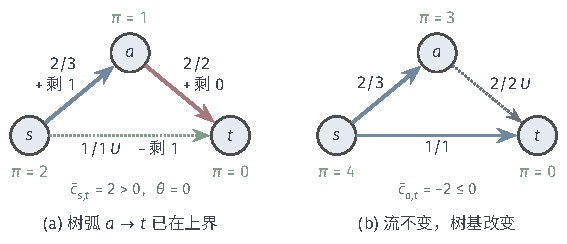
\includegraphics[width=96.054mm]{figures/01-basic-mathematics/04-graphs/tikz/c3-ns-degenerate/figure.pdf}
  \caption{退化换基。三点网络中$s\to t$的容量改为$1$，弧旁为流量与容量，“剩”为沿基本环调整方向的剩余量，绿色$\pi$为节点势。(a)入弧$s\to t$（绿色）在上界且约化费用为正，反向进入；树弧$a\to t$（红色）已在上界，剩余量为零，步长为零。(b)$a\to t$出基后流量与费用不变，新树基的势使全部非树弧满足最优性条件。}
  \label{fig:graph-opt-ns-degenerate}
\end{figure}

这个例子中的退化换基换来了一份最优性证书，但一般情形下，连续的零步长换基可能在若干个树基之间兜圈子，回到已经出现过的树基，费用始终不变，算法不再前进。因此，“费用不增加”本身不足以保证有限终止，阻塞弧有多条时选哪一条，必须写进算法。只取编号最小的弧不能排除循环，需要专门构造的规则。下面说明适用于有上下界弧的\term{词典序规则}（lexicographic rule）。

把上界写成等式$x_{i,j}+s_{i,j}=u_{i,j}$，$s_{i,j}\geq0$是上界松弛量。这样，每条弧有两个离界距离：$x_{i,j}-\ell_{i,j}$与$s_{i,j}$。非退化的情形是每条树弧的两个离界距离都为正，步长才一定为正。词典序规则用一个符号扰动人为地制造这种情形。在一个阶段开始时，把当前可行树基的树弧编号为$e_1,\ldots,e_{n-1}$，把$e_k$的流量改为$x_{e_k}+\sigma_k\varepsilon^k$：若$e_k$在上界取$\sigma_k=-1$，否则取$\sigma_k=+1$。供需随之改为扰动后流量所对应的净流出，并在整个阶段内保持不变；非树弧仍恰在界上。这里$\varepsilon$看作充分小的正数，每个量都表示成$(\text{常数},\varepsilon\text{的系数},\ldots,\varepsilon^{n-1}\text{的系数})$这样的向量，比较大小就是从常数项起按分量逐个比较，即词典序比较。于是每条树弧的两个离界距离在词典序下都严格为正。

每轮比较步长时，增加流量的树弧以向量$u-x(\varepsilon)$为候选，减少流量的树弧以$x(\varepsilon)-\ell$为候选，入弧以$(u-\ell,0,\ldots,0)$为候选，取词典序最小者作为步长$\theta(\varepsilon)$并让它出基。初始时各树弧的$\varepsilon$系数行是$\pm$单位向量，线性无关；每次换基，留下的树弧系数行加减出弧的系数行，入弧取出弧系数行的正负，这是可逆的行变换，界翻转则不改变系数行。所以各树弧的系数行始终线性无关，两条树弧的候选向量不会相等，入弧的候选向量与任一树弧也不会相等，词典序最小者唯一。更新后出弧恰好落在界上，其余树弧仍严格在界内，扰动后的问题始终非退化。

还原到基本环上，这个规则只在实际步长出现并列时起作用：比较并列阻塞弧的$\varepsilon$系数，选词典序最小的那条出基，实际流量仍按常数项更新。它为什么能防止循环，在下一小节的分析中说明。两个阶段各自从初始可行树基设置扰动：第一阶段从星形树基开始，第二阶段从清理人工结构后得到的树基重新开始。另一类常用规则要求维护所谓强可行树，它有自己的方向约定与初始化要求；第一阶段清理只保证得到普通的可行树基，不能据此断言原网络已经具有强可行树，这里不展开。

\paragraph{迭代算例}
回到图~\ref{fig:graph-opt-mcf-network}的三点网络，先做第一阶段。人工弧容量取总供给$3$，星形初始树为$s\to r$、$r\to t$、$a\to r$，流量依次为$3,3,0$，人工流总量为$6$，见图~\ref{fig:graph-opt-ns-artificial-start}(a)。按这个次序设置扰动，前两条树弧在上界，扰动后的流量为$3-\varepsilon$与$3-\varepsilon^2$，$a\to r$为$\varepsilon^3$。以$r$为根，第一阶段费用下的势为$(\pi_s,\pi_a,\pi_t,\pi_r)=(1,1,-1,0)$，非树弧$s\to t$与$a\to t$的约化费用都是$-2$。

\begin{figure*}[!htb]
  \centering
  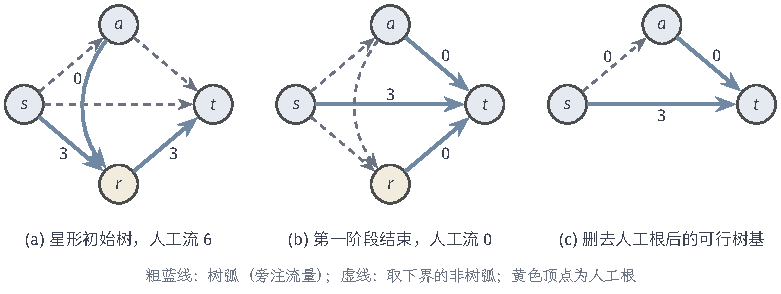
\includegraphics[width=132.186mm]{figures/01-basic-mathematics/04-graphs/tikz/c3-ns-artificial-start/figure.pdf}
  \caption{两阶段法的第一阶段。(a)增加人工根$r$（黄色），供给点、需求点和中转点分别用人工弧连向或连自$r$，得到显式可行的星形树，人工流总量为$6$。(b)两次换基后人工流降为零，原弧$s\to t$承担全部$3$单位，空载的人工弧$r\to t$仍在树中。(c)删去人工根和人工弧，剩下的树弧恰好构成原网络的生成树，作为第二阶段的初始可行树基。}
  \label{fig:graph-opt-ns-artificial-start}
\end{figure*}

选$s\to t$入弧。基本环上$s\to t$增加，$r\to t$与$s\to r$减少，剩余量依次为$4$、$3$、$3$，实际步长并列。两条并列弧的候选向量为$(3,0,-1,0)$与$(3,-1,0,0)$，后者词典序更小，所以$s\to r$出基。更新后$s\to t$承担$3$单位，人工流的常数部分已经为零。新势为$(-1,1,-1,0)$，$a\to t$的约化费用为$0-1+(-1)=-2$，再次入弧；这次$r\to t$与$a\to r$的剩余量都是$0$，是一次退化换基，比较$\varepsilon$系数后$a\to r$出基。此时全部非树弧满足条件，第一阶段最优值为零，见图~\ref{fig:graph-opt-ns-artificial-start}(b)。删去$r$后，树弧$s\to t$与$a\to t$已经构成原网络的生成树，$s\to a$在下界，这就是第二阶段的初始树基。

第二阶段从$T=\{s\to t,a\to t\}$、流量$(0,0,3)$开始，总费用为$12$。以$t$为根，逆着$s\to t$得$\pi_s=4$，逆着$a\to t$得$\pi_a=1$，势为$(4,1,0)$。非树弧$s\to a$在下界，约化费用为$1-4+1=-2<0$，选它正向入弧。基本环为$s\to a\to t$再逆着$s\to t$回到$s$：$s\to a$与$a\to t$增加，剩余量为$3$与$2$；$s\to t$减少，剩余量为$3$。步长$\theta=2$，由$a\to t$达到，费用下降$2\times2=4$。

$a\to t$到达上界，出基进入$U$，$s\to a$进入树。新流量为$(2,2,1)$，总费用为$8$。以$t$为根重新计算，$\pi_s=4$，顺着$s\to a$得$\pi_a=4-1=3$，势为$(4,3,0)$。唯一的非树弧$a\to t$在上界，约化费用为$1-3+0=-2\leq0$，满足条件，算法停止。这正是上一小节核对过的最优性证书。

再把$s\to a$的容量改为$1$，从同一初始树基出发。势与约化费用都不变，$s\to a$仍正向入弧，但三条弧的剩余量变为$1$、$2$、$3$，步长为$1$，由入弧自身达到。于是作界翻转：$s\to a$从$L$转入$U$，树不变，流量为$(1,1,2)$，费用为$10$。势仍为$(4,1,0)$，$s\to a$在上界，约化费用$-2\leq0$；没有其他非树弧，算法停止。逐项核对：$s$的净流出$1+2=3$，$a$的净流出$1-1=0$，$t$的净流出$-1-2=-3$，各弧流量都在界内。

图~\ref{fig:graph-opt-ns-pivots}把两种情形并排比较。两者从同一个树基、同一条入弧出发，只因入弧容量不同，阻塞弧一次是树弧、一次是入弧自身，分别对应树弧交换与界翻转。

\begin{figure*}[!htb]
  \centering
  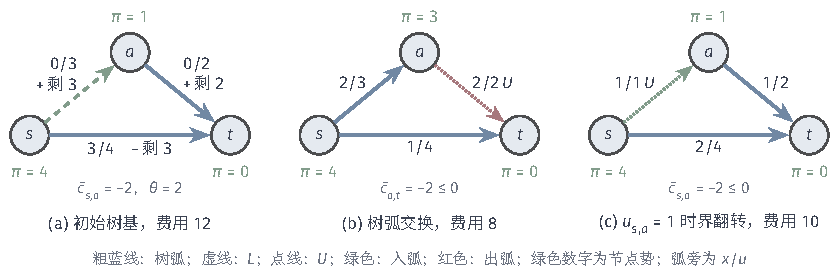
\includegraphics[width=142.053mm]{figures/01-basic-mathematics/04-graphs/tikz/c3-ns-pivots/figure.pdf}
  \caption{第二阶段的两种迭代。弧旁为流量与容量，“$+$剩”“$-$剩”为沿基本环增加或减少流量时的剩余量，$\pi$为节点势。(a)初始树基中$s\to a$的约化费用为$-2$，沿基本环最多推送$2$单位。(b)阻塞弧是树弧$a\to t$，它出基进入$U$，费用由$12$降为$8$。(c)若$s\to a$容量为$1$，入弧自身先到上界，树不变，费用降为$10$。两种结局中非树弧的约化费用都满足符号条件。}
  \label{fig:graph-opt-ns-pivots}
\end{figure*}

\subsection{算法分析与结果检验}
\label{sec:graph-opt-ns-analysis}

前面逐步说明了网络单纯形法的各个操作，本小节把它们合起来，回答三个问题：每轮迭代是否保持可行并改进费用，算法是否一定停止，停止时得到的是什么、要花多少计算。

\paragraph{可行性与费用变化}
每轮迭代沿基本环调整流量，环上每个顶点一进一出，各顶点的净流出不变；步长取环上各弧剩余量的最小值，所以调整后上下界仍然满足。树弧交换后新的$T$仍是生成树，出弧落在它所到达的界上，被正确归入$L$或$U$；界翻转只改变入弧的界状态。因此，每轮结束时都得到一个可行树基。费用的变化等于步长乘以入弧在调整方向上的约化费用，后者为负：步长为正时费用严格下降，步长为零时费用不变而树基改变。

\paragraph{有限终止}
仅凭费用不增不能推出有限终止，因为零步长的换基可能循环。词典序规则补上了这一缺口。在一个阶段内，扰动后的供需固定不变，扰动后的流量由树基$(T,L,U)$唯一确定，所以扰动后的费用（一个关于$\varepsilon$的多项式）是树基的函数。扰动后的问题非退化，每轮的步长$\theta(\varepsilon)$在词典序下严格为正，扰动后的费用便在词典序下严格下降，已经出现过的树基不可能再出现。可能的树基只有有限个：$T$是有限多棵生成树之一，每条非树弧只有两种界状态。所以每个阶段都在有限轮后停止。

停止时全部非树弧满足符号条件，树弧约化费用为零，由定理~\ref{thm:graph-opt-potential-certificate}，当前流在本阶段的费用下最优。对第一阶段，这给出可行性的判定；对第二阶段，这给出原问题的最优流。以上论证都假设精确运算。

\paragraph{单轮开销}
设顶点数为$n$，弧数为$a$。朴素实现每轮扫描全部非树弧计算约化费用，需要$O(a)$次运算；为树记录父顶点与深度后，从入弧两端沿父指针上溯到最近公共祖先即可找出基本环，并沿环比较剩余量、更新流量，都是$O(n)$；沿新树重新计算势也是$O(n)$。所以每轮为$O(n+a)$次运算，只扫描部分弧的定价策略可以降低这一项。总开销还取决于迭代轮数，其中包括退化换基。上面的有限性论证只给出与树基个数相当的上界，不能从每轮简单推出总运算量具有统一的多项式界；本书也不据此断言网络单纯形法一定快于专门的最大流或指派算法。

\paragraph{结果检验}
输出须回到原始问题检查：先把下界平移量加回流量，核对每个顶点的净流出等于原始$b_i$、每条弧满足原始上下界，再按原始费用重算目标值，并确认它等于平移后问题的费用加上常数$\bm c^{\top}\bm\ell$。最优性则逐弧核对势条件~\eqref{eq:graph-opt-mcf-certificate}。浮点实现中，守恒误差、界约束误差与约化费用的符号都只能在容差内判断，应分别报告；近似满足的条件说明结果接近最优，不能直接当作精确证书。

\paragraph{与其他问题的关系}
最大流与最小费用流使用同一种残量网络，但改进方式不同：最大流沿源汇之间的增广路径增加输送量，最小费用流在供需固定时沿环调整流量以减少费用。下一节的匹配可以写成单位容量的最大流，第~\ref{sec:graph-assignment}节的指派则可以写成单位容量的最小费用流。尽管如此，后面两节仍分别介绍专门的增广算法：一般模型说明问题之间可以互相转写，专门算法则利用二部配对的结构，状态更简单，开销也有更直接的界。

% 第3章第5节：匹配（二部图匹配问题；交替路径、单位容量网络与最优性条件；增广匹配算法；算法分析与结果检验）。

\section{匹配}
\label{sec:graph-matching}

把若干任务分给若干名人员，每人至多接一项任务，每项任务至多由一人完成，而且只有具备相应资格的人才能接某项任务。目标是让完成配对的任务尽可能多。这里选择的对象是一组“人员—任务”配对，约束是任何人员或任务都不能出现在两个配对中。

本节先给出二部图匹配的定义，并用小例子区分“无法直接再加边”与“边数最多”。随后以交替路径建立改进机制：沿一条两端都未配对的交替路径翻转选边状态，配对数就增加一；借助单位容量的流网络，第~\ref{sec:graph-max-flow}节的最大流判据给出相应的最大性条件。最后把这一机制写成增广匹配算法，分析开销并说明怎样验收结果。本节只比较配对的数量，不涉及配对的成本。

\subsection{二部图匹配问题}
\label{sec:graph-opt-match-problem}

人员与任务分属两类对象，资格关系只连接一名人员与一项任务，同类对象之间没有边。若无向图的顶点集能分成两个不相交的部分$U$与$W$，使每条边都恰有一个端点在$U$、另一个端点在$W$，就称它为\term{二部图}（bipartite graph），记作$\mathcal G=(U\cup W,E)$。本节称$U$为左侧、$W$为右侧，两侧的顶点数可以不同。

\begin{definition}[匹配]
\label{def:graph-opt-matching}
图$\mathcal G=(V,E)$中两两没有公共端点的边组成的集合$M\subseteq E$称为一个\term{匹配}（matching）。$M$中某条边的端点称为被$M$饱和，其余顶点称为自由顶点。饱和全部顶点的匹配称为\term{完美匹配}（perfect matching）。不能再加入任何一条边而仍为匹配的$M$称为\term{极大匹配}（maximal matching），边数最多的匹配称为\term{最大匹配}（maximum matching）。
\end{definition}

最大匹配一定是极大匹配，反过来不成立。图~\ref{fig:graph-opt-match-maximal-maximum}中允许边为$a-x$、$a-y$、$b-x$。若先选了$a-x$，$a$与$x$都已被占用，剩下的两条边各与它共享一个端点，无法再加，所以$\{a-x\}$是极大匹配；但$\{a-y,b-x\}$有两条边，是最大匹配，也是完美匹配。从$\{a-x\}$到$\{a-y,b-x\}$，靠的不是继续加边，而是把$a$的配对从$x$改到$y$，腾出$x$给$b$。这说明逐条贪心加边可能停在较差的结果上，重排已有配对才是改进的关键。

\begin{figure}[!htb]
  \centering
  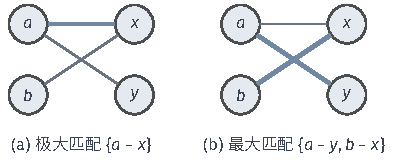
\includegraphics[width=67.07mm]{figures/01-basic-mathematics/04-graphs/tikz/c3-match-maximal-maximum/figure.pdf}
  \caption{极大匹配与最大匹配。细线为允许的配对，粗蓝线为选中的匹配边。(a)$\{a-x\}$已无法再加入任何边，是极大匹配；(b)$\{a-y,b-x\}$的边数更多，是最大匹配。由(a)到(b)须改动已有的配对$a-x$。}
  \label{fig:graph-opt-match-maximal-maximum}
\end{figure}

本节的目标只是最大化$|M|$，边上没有费用；要求完成配对并比较成本的问题留到第~\ref{sec:graph-assignment}节。两侧大小不同时，最大匹配至多有$\min\{|U|,|W|\}$条边，但未必达到这个数：若左侧两个顶点都只与右侧同一个顶点相连，无论怎样选，至多只有一个能配上。下面的构造还依赖两侧的划分。一般的无向图可能含有奇数长的环，例如三角形，它的顶点无法分成两侧使每条边跨侧，下面的单位容量网络构造对它不适用，一般图的匹配需要另外的机制。

\subsection{交替路径与最优性条件}
\label{sec:graph-opt-match-alternating}

图~\ref{fig:graph-opt-match-maximal-maximum}中的改进可以这样描述：从自由顶点$b$出发，先走未选的边$b-x$，再走已选的边$x-a$，最后走未选的边$a-y$到达自由顶点$y$，然后把这条路径上每条边的选中状态取反。下面把这一操作一般化。

给定匹配$M$，若一条路径上的边交替地不属于$M$与属于$M$，称它为\term{交替路径}（alternating path）。两个端点都是自由顶点的交替路径称为关于$M$的增广路径。增广路径的首尾两条边都不在$M$中，因为端点自由；所以路径上不在$M$中的边比在$M$中的边恰好多一条。

\begin{lemma}[沿增广路径翻转]
\label{lem:graph-opt-match-flip}
设$P$是关于匹配$M$的增广路径，把$P$上属于$M$的边移出、不属于$M$的边加入，得到的边集$M'$仍是匹配，且$|M'|=|M|+1$。
\end{lemma}

\begin{proof}
不在$P$上的顶点所关联的选边没有变化。$P$的内部顶点在翻转前恰关联$P$上的一条匹配边和一条非匹配边，翻转后两者互换，仍恰关联一条选边；它不会关联$P$以外的匹配边，因为它在$M$中的唯一配对已经在$P$上。$P$的两个端点原来是自由的，翻转后各关联一条选边。所以$M'$中没有两条边共享端点。由于$P$上非匹配边比匹配边多一条，$|M'|=|M|+1$。
\end{proof}

\paragraph{单位容量网络}
增广路径与第~\ref{sec:graph-max-flow}节的增广路径同名，并非巧合。由二部图构造流网络：增加源点$s$与汇点$t$，从$s$向每个$u\in U$连容量为$1$的弧，每条允许边$u-w$改为容量为$1$的弧$u\to w$，再从每个$w\in W$向$t$连容量为$1$的弧。图~\ref{fig:graph-opt-match-flow-network}画出了一个这样的网络。

给定匹配$M$，在每条匹配边$u-w$对应的路线$s\to u\to w\to t$上各送一单位，得到流值为$|M|$的整数流。反过来，设$\bm x$是一个整数流，每条弧的流量只能是$0$或$1$。顶点$u\in U$只有一条容量为$1$的入弧，流守恒使它至多有一条流量为$1$的出弧；同理，每个$w\in W$至多有一条流量为$1$的入弧。所以流量为$1$的中间弧对应的边两两不共享端点，构成一个匹配，边数等于流值。整数流与匹配就这样一一对应，并且流值等于边数。不能用分数流量四舍五入来代替这一对应：分数流不直接给出配对。

在这个对应下，残量网络中的$s$到$t$简单路径恰好是增广路径。设$\bm x$对应匹配$M$。从$s$出发，正向残量弧$s\to u$存在当且仅当$u$自由；从左侧顶点$u$，可以沿正向残量弧走到任一个与$u$由非匹配边相连的$w$；从右侧顶点$w$，若$w$自由可以走$w\to t$到达汇点，否则只能沿反向残量弧$w\to u'$回到它的配对$u'$，相当于准备撤回匹配边$u'-w$。所以这样一条路径依次经过一个自由左侧顶点、交替的非匹配边与匹配边、一个自由右侧顶点，沿它增广恰好就是引理~\ref{lem:graph-opt-match-flip}中的翻转。

\begin{figure}[!htb]
  \centering
  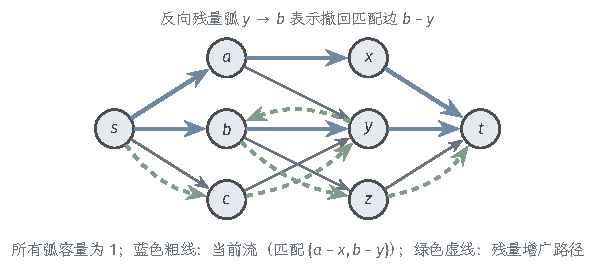
\includegraphics[width=100.76mm]{figures/01-basic-mathematics/04-graphs/tikz/c3-match-flow-network/figure.pdf}
  \caption{二部图匹配的单位容量网络。允许边为$a-x,a-y,b-y,b-z,c-y$，全部弧容量为$1$。蓝色粗弧是匹配$\{a-x,b-y\}$对应的流，流值为$2$。绿色虚线是残量网络中的一条$s$到$t$路径，其中$y\to b$是反向残量弧，表示撤回匹配边$b-y$；这条路径对应交替路径$c-y-b-z$。}
  \label{fig:graph-opt-match-flow-network}
\end{figure}

\paragraph{最大性条件}
有了上面的对应，最大流的判据可以直接搬到匹配上。

\begin{theorem}[增广路径判据]
\label{thm:graph-opt-match-augmenting}
二部图中的匹配$M$是最大匹配，当且仅当不存在关于$M$的增广路径。
\end{theorem}

\begin{proof}
若存在增广路径，由引理~\ref{lem:graph-opt-match-flip}可得更大的匹配，$M$不是最大的。反过来，设不存在增广路径，令$\bm x$是$M$对应的流。由上面的对应，$\bm x$的残量网络中没有$s$到$t$的路径，由第~\ref{sec:graph-max-flow}节的增广路径判据，$\bm x$是最大流。任何匹配$M''$对应一个流值为$|M''|$的流，所以$|M''|\leq\operatorname{val}(\bm x)=|M|$，$M$是最大匹配。
\end{proof}

整数容量时Ford--Fulkerson方法输出整数最大流，所以最大流值总能由某个匹配达到，最大流值就等于最大匹配的边数。

判据与“不能再加一条边”的区别，可以在图~\ref{fig:graph-opt-match-augment}上看清。允许边为$a-x$、$a-y$、$b-y$、$b-z$、$c-y$，当前匹配为$\{a-x,b-y\}$。剩下的三条边$a-y$、$b-z$、$c-y$都与已选边共享端点，所以这个匹配是极大的。但从自由顶点$c$出发，走非匹配边$c-y$、匹配边$y-b$、非匹配边$b-z$，到达自由顶点$z$，得到增广路径$c-y-b-z$。翻转后撤去$b-y$，加入$c-y$与$b-z$，匹配变为$\{a-x,b-z,c-y\}$，大小由$2$增为$3$。

\begin{figure*}[!htb]
  \centering
  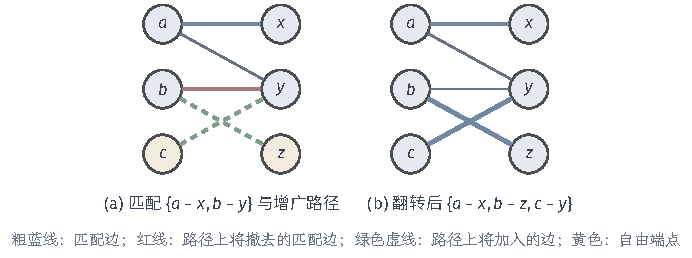
\includegraphics[width=117.094mm]{figures/01-basic-mathematics/04-graphs/tikz/c3-match-augment/figure.pdf}
  \caption{沿交替路径翻转。(a)匹配$\{a-x,b-y\}$是极大匹配，但自由顶点$c$与$z$（黄色）之间有增广路径$c-y-b-z$：绿色虚线为路径上将加入的非匹配边，红线为将撤去的匹配边。(b)翻转后$a-x$保留，$b-y$被$b-z$与$c-y$取代，配对数增加一。}
  \label{fig:graph-opt-match-augment}
\end{figure*}

\subsection{增广匹配算法}
\label{sec:graph-opt-match-algorithm}

定理~\ref{thm:graph-opt-match-augmenting}给出一个算法：只要存在增广路径就沿它翻转，不存在时停止。剩下的问题是怎样在二部图上直接搜索增广路径，而不必显式建立流网络。

算法维护的状态包括：两侧每个顶点的配对伙伴（自由顶点记为空），以及每轮搜索使用的访问标记和右侧顶点的前驱。每轮搜索同时从所有自由左侧顶点出发，用一个队列作广度优先遍历。从左侧顶点$u$出发时，检查它的每个邻居$w$：若$w$尚未访问，则标记$w$并记前驱为$u$；这时若$w$自由，就找到了增广路径，否则把$w$的配对伙伴放入队列，相当于沿匹配边从$w$回到左侧。队列耗尽仍未到达自由右侧顶点，说明当前不存在增广路径。这一搜索恰好就是在单位容量网络的残量网络中从$s$出发的遍历，只是省去了$s$与$t$。

找到自由右侧顶点$w$后，沿前驱回溯：$w$的前驱是左侧顶点$u$，若$u$不自由，再从$u$的原配对伙伴继续回溯，直到到达作为出发点的自由左侧顶点。回溯得到的就是一条增广路径，沿它统一翻转配对伙伴。搜索过程中匹配保持不变，只有完整找到增广路径之后才修改，这样前驱链始终描述同一个匹配下的交替路径。

\begin{algorithm}[增广匹配]
\label{alg:graph-opt-augmenting-matching}
输入：二部图$\mathcal G=(U\cup W,E)$的邻接表。输出：最大匹配$M$，以及最后一次失败搜索的已访问顶点集。状态：两侧顶点的配对伙伴、访问标记、右侧顶点的前驱、队列。
\begin{enumerate}
  \item 令$M=\varnothing$，全部配对伙伴为空。
  \item 清除访问标记，把所有自由左侧顶点放入队列并标记。
  \item 逐个取出左侧顶点$u$，对每个未访问的邻居$w$作标记并令其前驱为$u$；若$w$自由，转第4步，否则把$w$的配对伙伴标记后放入队列。队列耗尽时转第5步。
  \item 从$w$沿前驱与原配对伙伴交替回溯到一个自由左侧顶点，沿这条增广路径翻转配对伙伴，回到第2步。
  \item 输出$M$与本轮的已访问顶点集，停止。
\end{enumerate}
\end{algorithm}

\paragraph{算例}
在图~\ref{fig:graph-opt-match-augment}的二部图上，从$M=\{a-x,b-y\}$开始。自由左侧顶点只有$c$。从$c$检查邻居$y$，记前驱$y\leftarrow c$；$y$已与$b$配对，把$b$放入队列。从$b$检查邻居：$y$已访问，$z$未访问，记前驱$z\leftarrow b$，而$z$自由，找到增广路径。回溯：$z$的前驱是$b$，$b$原来配$y$，$y$的前驱是$c$，$c$自由，路径为$c-y-b-z$。翻转后$c$配$y$，$b$配$z$，$a$仍配$x$，得到大小为$3$的匹配。

下一轮开始时已没有自由左侧顶点，队列一开始就是空的，搜索立即失败，算法停止。这时$|M|=3=|U|$，结论也可以直接从上界看出。若把边$b-z$删去，情形就不同了：从$c$到$y$，再沿匹配边到$b$，$b$的邻居只有已访问的$y$，队列耗尽，不存在增广路径，匹配$\{a-x,b-y\}$就是最大匹配。这里虽然仍有自由顶点$c$与$z$，但不存在连接它们的交替路径，所以不能再改进。对应的残量网络中，从$s$可达的顶点集为$\{s,c,y,b\}$，跨出这一集合的弧是满流的$s\to a$与$y\to t$，割容量为$2$，等于匹配的边数。

\subsection{算法分析与结果检验}
\label{sec:graph-opt-match-analysis}

\paragraph{计算开销}
记$n=|U|+|W|$，$m$为允许边数，$\nu=\min\{|U|,|W|\}$。每次成功的翻转使匹配增加一条边，而匹配至多有$\nu$条边，所以成功的搜索不超过$\nu$次，再加上最后一次失败的搜索。一轮搜索中每个顶点至多入队或标记一次，每条边至多从它的左端点检查一次，所以搜索为$O(n+m)$；回溯与翻转沿一条路径进行，为$O(n)$；初始化配对数组为$O(n)$。总运算量为$O(\nu(n+m))$。还有按层同时寻找多条增广路径的更快的匹配算法，本书不展开，也不引用它们的复杂度界。

\paragraph{结果检验}
检验分两步。可行性：逐条核对所选边都是允许边、任意两条所选边没有公共端点，再重新数出边数。最大性：可以重做一次从全部自由左侧顶点出发的交替搜索，确认到达不了自由右侧顶点；也可以用最后一次失败搜索的已访问顶点集加上$s$构造单位容量网络中的割，核对割容量等于匹配边数，这是一份不依赖算法过程的证书。不能因为每个自由左侧顶点都不与自由右侧顶点直接相连就宣布最大，图~\ref{fig:graph-opt-match-augment}(a)正是这种情形，而那里仍有增广路径。

% 第3章第6节：指派（指派问题与模型变形；可行标号与紧边证书；匈牙利算法；算法分析、结果检验与问题比较）。

\section{指派}
\label{sec:graph-assignment}

上一节只关心能配上多少对。现在每个对象都必须完成配对，而不同配对的成本不同：把$N$项工作分给$N$名工人，每人做一项，工人$i$做工作$j$的耗时为$c_{i,j}$，要使总耗时最少。可行解仍是二部图中的匹配，而且必须是完美匹配；新增的是边上的成本，以及证明一个解已经最省的手段。

本节先写出指派问题及几种常见变形。随后给行与列配置标号，用它们给出任何完整指派成本的下界，并说明只用“紧边”完成的指派恰好达到这个下界。匈牙利算法同时维护可行标号与由紧边组成的匹配：匹配用上一节的交替路径扩大，扩大不了时调整标号以产生新的紧边。最后分析开销，说明怎样检验结果，并比较最大匹配、指派与最小费用流三种问题。

\subsection{指派问题}
\label{sec:graph-opt-assign-problem}

把工人看成左侧的行，工作看成右侧的列。行$i$与列$j$之间允许配对时，配对成本$c_{i,j}$是有限实数；不允许的配对没有边。

\begin{definition}[指派问题]
\label{def:graph-opt-assignment}
设有$N$行、$N$列，允许的行列对组成边集$E$，每条边$(i,j)\in E$有有限实成本$c_{i,j}$。\term{指派问题}（assignment problem）要求选出一个完美匹配，即给每行指定一个不同的列，并且只用允许边，使总成本$\sum_i c_{i,\sigma(i)}$最小，其中$\sigma(i)$是分给行$i$的列。
\end{definition}

全部行列对都允许时，$\sigma$可以是任意置换，用$0$-$1$变量$x_{i,j}$表示就是每行每列恰选一个元素。行数少于列数的矩形情形，可以补充若干虚拟行，它们到每一列的成本都是零：补成方阵后，虚拟行只占用原来没有被真实行使用的列，总成本不变，删去虚拟行的配对就得到原问题的解。

实际问题中还要分清三种设定。第一种是本节主线，每个对象都必须配对。第二种允许不配对，但未配对要付惩罚。这时不能只把“恰选一次”放宽成“至多选一次”：成本都非负时，什么都不选的空匹配就成了最优解。正确的做法是把惩罚写进模型，例如给每个左侧对象$i$配一个专属虚拟列，配给它的成本是$i$的惩罚$\rho_i$；给每个右侧对象$j$配一个专属虚拟行，成本是$j$的惩罚$\eta_j$；真实对象与非专属虚拟对象之间禁止配对，虚拟行与虚拟列之间成本为零。这样补成的方阵中，完整指派的成本恰为真实配对成本加上未配对对象的惩罚。第三种设定是某些配对被禁止，这由边集$E$表达。若某一行没有任何允许边，或者一组行能使用的列总数少于行数，就不存在完美匹配，必须报告不可行，而不是给出一个使用禁止配对的“解”。

指派也可以写成上一节与第~\ref{sec:graph-min-cost-flow}节的模型：令每行供给$1$、每列需求$1$，每条允许边是容量为$1$、单位费用为$c_{i,j}$的弧，则整数可行流与完美匹配一一对应，费用就是指派成本。由树流的整数性，网络单纯形法在这个网络上给出的最优流是整数流，所以可以直接用它求解。尽管如此，本节仍利用二部配对的结构设计专门算法：模型之间可以转换，并不意味着必须采用同一个求解过程。

\subsection{可行标号与最优性条件}
\label{sec:graph-opt-assign-labels}

最小费用流用节点势给出最优性证书。在指派问题中，同样的思想可以写得更直接：给每行、每列各配一个数，用它们给出任意完整指派成本的一个下界。以下设问题已补成$N$阶方阵，每行每列恰配一次。

给每行$i$配实数$u_i$，每列$j$配实数$v_j$。若对每条允许边都有
\begin{equation}
  u_i+v_j\leq c_{i,j},
  \label{eq:graph-opt-feasible-labels}
\end{equation}
就称$(\bm u,\bm v)$为\term{可行标号}（feasible labeling）。对任意完整指派$\sigma$，把它用到的$N$条边的不等式相加，每行恰出现一次、每列也恰出现一次，于是
\[
  \sum_{i=1}^Nc_{i,\sigma(i)}\geq\sum_{i=1}^N\bigl(u_i+v_{\sigma(i)}\bigr)=\sum_{i=1}^Nu_i+\sum_{j=1}^Nv_j.
\]
右边与$\sigma$无关，是全部完整指派成本的共同下界。这个论证只依赖“每行每列恰计一次”，不需要一般的线性规划对偶理论。在上一小节的流模型中把$\pi_i=u_i$、$\pi_j=-v_j$看成节点势，$c_{i,j}-u_i-v_j$就是行到列弧的约化费用，可行标号对应全部约化费用非负。

使式~\eqref{eq:graph-opt-feasible-labels}取等号的边称为\term{紧边}（tight edge），$c_{i,j}-u_i-v_j$称为边的剩余量。

\begin{theorem}[紧边指派的最优性]
\label{thm:graph-opt-tight-assignment}
设$(\bm u,\bm v)$是可行标号。若完整指派$\sigma$只使用紧边，则它的成本等于$\sum_iu_i+\sum_jv_j$，因而是最优指派。
\end{theorem}

\begin{proof}
$\sigma$用到的每条边都取等号，上面的求和不等式也取等号，所以$\sigma$的成本等于下界。任何完整指派的成本都不低于这个下界，所以$\sigma$最优。
\end{proof}

于是求解指派问题的任务变成两件同时进行的事：保持标号可行，同时在紧边中寻找完美匹配。可行标号本身只提供下界；在找到全由紧边组成的完整指派之前，不能宣称已经得到最优解。

\subsection{匈牙利算法}
\label{sec:graph-opt-hungarian}

\term{匈牙利算法}（Hungarian algorithm）从一组容易得到的可行标号和空匹配出发，只在紧边上扩大匹配；当紧边不够用时，修改标号以制造新的紧边，同时保证已有的紧边匹配不被破坏。

\paragraph{初始可行标号}
先检查每行至少有一条允许边，否则直接报告不可行。取每行的最小允许成本作为行标号$u_i=\min_{j:\,(i,j)\in E}c_{i,j}$，列标号全取零。每条允许边满足$u_i+0\leq c_{i,j}$，标号可行，并且每行至少有一条紧边。

\paragraph{交替树的生长}
从一个自由行出发，在紧边上用上一节的交替搜索建立\term{交替树}（alternating tree）：从行出发只走紧的非匹配边到列；若到达的列已经匹配，就沿匹配边回到它的配对行，继续扩展；若到达自由列，从树根到该列的路径就是一条由紧边组成的增广路径，沿它翻转，匹配增加一条边，然后从下一个自由行重新建树。树中每个列都与树中某一行匹配，每个非根行都是从它的配对列走进来的，所以若记树中的行集为$S$、列集为$T$，则$|S|=|T|+1$，多出的一行就是自由的树根。

\paragraph{标号调整}
如果交替树不能再扩展，说明从$S$出发的紧边都通向$T$。这时在$S$到树外列的允许边中求最小剩余量
\begin{equation}
  \delta=\min\bigl\{c_{i,j}-u_i-v_j:\ i\in S,\ j\notin T,\ (i,j)\in E\bigr\},
  \label{eq:graph-opt-hungarian-delta}
\end{equation}
并令$S$中各行的标号加$\delta$、$T$中各列的标号减$\delta$。由于树外的这些边都不紧，$\delta>0$。逐类检查这一调整的效果。两端分别在$S$与$T$中的边，$u_i+v_j$不变，树中的紧边和匹配边都保持紧，交替树完整保留。行在$S$、列不在$T$的边，剩余量减少$\delta$，由$\delta$的取法仍然非负，取到最小值的边变成紧边，于是交替树至少可以多扩展一步。行不在$S$、列在$T$的边，剩余量增加$\delta$；其余的边不变。匹配边要么两端都在树中，要么两端都在树外，所以全部保持紧。调整后标号仍然可行，而标号下界$\sum u_i+\sum v_j$增加了$|S|\delta-|T|\delta=\delta$。

若式~\eqref{eq:graph-opt-hungarian-delta}中的候选集合为空，$S$中各行的允许列全部落在$T$中，$|S|$行只能使用$|T|=|S|-1$个列，不可能各配一个不同的列，于是报告不可行，而不是虚构一个有限的步长。

\begin{algorithm}[匈牙利算法]
\label{alg:graph-opt-hungarian}
输入：$N$阶方阵形式的指派问题（允许边集与成本）。输出：最优完整指派与可行标号，或“不可行”的结论。状态：行列标号、紧边匹配、交替树的行集$S$与列集$T$、各列的前驱、未入树列的最小剩余量。
\begin{enumerate}
  \item 若某行没有允许边，报告不可行；否则取$u_i$为第$i$行最小允许成本、$v_j=0$，匹配为空。
  \item 若所有行都已匹配，转第5步；否则取一个自由行作为交替树的根，令$S$只含它、$T=\varnothing$。
  \item 从$S$中的行沿紧的非匹配边扩展到列，已匹配的列沿匹配边把它的配对行加入$S$。若到达自由列，沿前驱翻转增广路径，回到第2步。
  \item 若树不能再扩展：候选集合为空则报告不可行；否则按式~\eqref{eq:graph-opt-hungarian-delta}求$\delta$，$S$中行标号加$\delta$、$T$中列标号减$\delta$，回到第3步。
  \item 输出匹配与标号；若曾补充虚拟行或虚拟列，按原始模型删去或解释相应配对。
\end{enumerate}
\end{algorithm}

在整个过程中，有三条性质始终保持：标号可行，匹配只用紧边，交替树中的边都是紧边。增广只改变匹配，不改变标号；调标号只改变标号，不破坏已有的紧边匹配与交替树。全部行都匹配时，匹配是一个只由紧边组成的完整指派，由定理~\ref{thm:graph-opt-tight-assignment}，它是最优的。所以这个算法不只是一串对成本矩阵的减法操作，每一步都维护着一份可以随时核对的下界。

\paragraph{算例}
成本矩阵为
\[
  \bm C=\begin{bmatrix}1&2\\1&100\end{bmatrix}.
\]
逐行贪心时，第一行先取最便宜的第$1$列，成本$1$，第二行只剩第$2$列，成本$100$，合计$101$。另一种指派是第一行配第$2$列、第二行配第$1$列，成本为$2+1=3$。贪心的问题在于两行都最偏爱第$1$列，而第二行失去它的代价远大于第一行。

匈牙利算法取初始标号$u=(1,1)$、$v=(0,0)$，紧边为$(1,1)$与$(2,1)$。第一行沿紧边到达自由的第$1$列，直接配对。第二行出发建树：沿紧边到第$1$列，第$1$列已配给第一行，把第一行加入树；第一行的紧边只有到第$1$列的那一条，树无法扩展，如图~\ref{fig:graph-opt-hungarian}(a)。此时$S=\{1,2\}$，$T=\{1\}$，树外列只有第$2$列，剩余量分别为$c_{1,2}-u_1-v_2=1$与$c_{2,2}-u_2-v_2=99$，所以$\delta=1$。

调整后$u=(2,2)$、$v=(-1,0)$。边$(1,1)$与$(2,1)$的剩余量仍为零，边$(1,2)$的剩余量变为$2-2-0=0$，成为新的紧边，边$(2,2)$的剩余量为$98$。交替树从第一行扩展到自由的第$2$列，得到增广路径：第二行—第$1$列—第一行—第$2$列，如图~\ref{fig:graph-opt-hungarian}(b)。翻转后第二行配第$1$列，第一行配第$2$列，成本为$2+1=3$；标号下界为$2+2+(-1)+0=3$，两者相等，图~\ref{fig:graph-opt-hungarian}(c)的指派最优。

\begin{figure}[!htb]
  \centering
  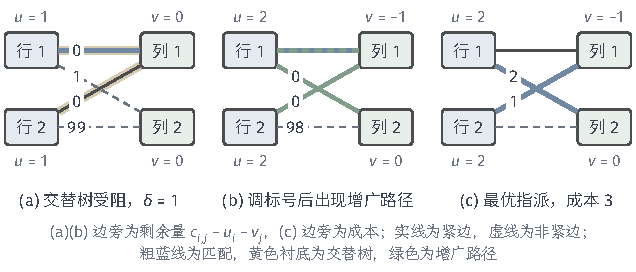
\includegraphics[width=107.714mm]{figures/01-basic-mathematics/04-graphs/tikz/c3-assign-hungarian/figure.pdf}
  \caption{匈牙利算法在成本矩阵$\left[\begin{smallmatrix}1&2\\1&100\end{smallmatrix}\right]$上的运行。行、列旁为当前标号。(a)匹配为行$1$配列$1$，从自由的行$2$出发的交替树（黄色衬底）只到达列$1$与行$1$，树外边的最小剩余量为$\delta=1$。(b)行标号加$1$、树中列标号减$1$后，行$1$到列$2$变紧，出现增广路径（绿色）。(c)翻转得到的指派成本为$3$，等于标号之和。}
  \label{fig:graph-opt-hungarian}
\end{figure}

\paragraph{停止与还原}
全部行都匹配后停止。若为矩形问题补过零成本虚拟行，删去它们的配对即得原问题的解；若按惩罚模型补过专属虚拟行列，配给专属虚拟对象的真实对象就是未配对的对象，总成本中相应的项就是它的惩罚。禁止的配对从未作为允许边出现，所以不会出现在结果中。

\subsection{算法分析与结果检验}
\label{sec:graph-opt-assign-analysis}

\paragraph{计算开销}
朴素地实现，每次调标号都要扫描$S$中全部行到树外全部列的剩余量。更好的做法是为每个未入树的列$j$维护最小剩余量$\min_{i\in S}(c_{i,j}-u_i-v_j)$及取到最小值的行，作为这一列的前驱。有一行加入$S$时，用它到各列的剩余量更新这些最小值，花$O(N)$；求$\delta$只需在这些最小值中再取最小，花$O(N)$；调标号后，未入树列的最小剩余量统一减去$\delta$，也是$O(N)$。为一个自由行建树直到增广，至多有$N$行加入$S$、至多调标号$N$次，所以一次增广为$O(N^2)$；至多增广$N$次，稠密$N$阶方阵上的总运算量为$O(N^3)$次实数运算。存储上，原始成本表占$N^2$个数，这是输入本身；算法额外的工作数组为$O(N)$。

\paragraph{结果检验}
先检查原始问题的可行性：每行恰配一个列，所用的列互不相同，全部配对都是允许边；再按原始成本重算总成本。然后检查证书：对全部允许边验证$u_i+v_j\leq c_{i,j}$，对所选的边验证取等号，并核对总成本等于$\sum_iu_i+\sum_jv_j$。原始可行解的成本等于标号下界，才构成最优性证书。浮点实现中，“紧”与“可行”都只能在容差内判断，应说明所用容差；近似相等不能无条件替代精确证书。

\paragraph{三种问题的比较}
最大匹配、指派与最小费用流可以互相转写，但目标与约束不同。最大匹配只求配对数量，边上没有成本；指派要求每个对象都完成配对，在这一条件下比较成本；最小费用流允许一般的容量、上下界与供需，指派只是全部容量为一、每行供给一、每列需求一的特例。图~\ref{fig:graph-opt-problem-relations}汇总了这些关系。专门算法保留了各自的结构：增广匹配只需记录配对伙伴，匈牙利算法的标号与交替树都利用了二部结构，网络单纯形法则适用于一般网络。算法名称不是不改模型就能互换的工具，换用另一种算法之前，须先把问题按它的输入要求重新写出。

\begin{figure}[!htb]
  \centering
  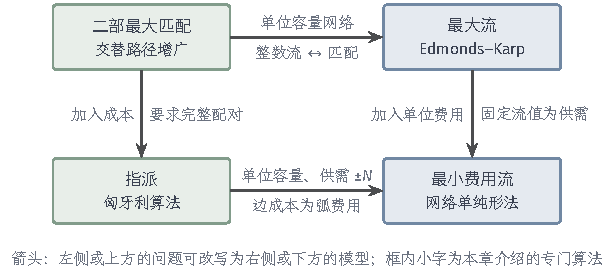
\includegraphics[width=103.914mm]{figures/01-basic-mathematics/04-graphs/tikz/c3-problem-relations/figure.pdf}
  \caption{本章四种流与配对问题之间的模型关系。箭头表示起点的问题可以写成终点的模型：二部最大匹配是单位容量的最大流，加入成本并要求完整配对就成为指派；最大流固定流值并加入单位费用就成为最小费用流，指派是单位容量的最小费用流。框内小字是本章为各问题介绍的专门算法。}
  \label{fig:graph-opt-problem-relations}
\end{figure}

% 第3章第7节：本章小结。

\section{本章小结}
\label{sec:graph-optimization-summary}

本章的六个问题都在有限图上从满足结构要求的候选中挑选数值最好者，但选择的对象和数值的含义各不相同。最短路选一条路径，比较弧长之和；最小生成树选一组连接全部顶点的边，比较建造成本之和；最大流给每条弧分配流量，在容量上界内最大化源汇之间的净输送量；最小费用流在供需固定时比较输送费用；匹配选互不共享端点的边，只数配对个数；指派要求每个对象都完成配对，再比较配对成本。同样写在边旁的一个数，可以是长度、成本、容量或单位费用，它们不能互换解释：例如最小生成树上两点间的路径未必是最短路，最大流也不关心沿哪条路线输送更便宜。

各算法依靠的论证与成立条件也不同。有向无环图上的递推依靠拓扑序，前驱的距离在使用前已经确定；Bellman--Ford算法允许负边长，靠“至多$k$条弧”的递推反复修正标签，并能识别负环的影响；Dijkstra算法只在边长非负时成立，每次永久确定一个顶点。Kruskal算法与Prim算法依靠割性质，用交换论证说明每次选的边可以留在某棵最优树中。最大流的Ford--Fulkerson方法与Edmonds--Karp算法沿残量网络中的增广路径增加流量，前者在整数容量下有限终止，后者按最少弧数选路，对实容量也给出增广次数的界。网络单纯形法沿树上的基本环调整流量，靠词典序规则排除零步长换基造成的循环。增广匹配沿交替路径翻转选边状态；匈牙利算法在紧边上增广，在受阻时调整标号。

许多算法停止时都留下一份可以独立核对的证书，表~\ref{tab:graph-opt-summary}把它们与输入条件、主要开销并列。最短路的证书是逐弧距离不等式；最大流的证书是同值的流与割；最小费用流的证书是流量与节点势满足的逐弧符号条件；最大匹配的证书是单位容量网络中与匹配边数同值的割；指派的证书是成本等于标号之和的紧边指派。最小生成树的最优性则回到割性质：每条非树边都不轻于它在树上所对应路径中的边。证书的价值在于检查者不必相信求解过程，只需核对可行性和若干不等式；浮点计算中这些核对都要带容差，近似满足不能直接当作精确证书。

\begin{table*}[!htb]
  \centering\small
  \caption{本章六个问题的对比（$n$为顶点数，$m$为无向边数，$a$为有向弧数，$\nu$为二部图较小一侧的顶点数，$N$为指派方阵的阶数）。开销均为本章所述实现的运算量。}
  \label{tab:graph-opt-summary}
  \begin{tabularx}{\linewidth}{@{}l>{\raggedright\arraybackslash}X>{\raggedright\arraybackslash}X>{\raggedright\arraybackslash}X>{\raggedright\arraybackslash}p{30mm}@{}}
    \toprule
    问题 & 选择对象与目标 & 方法与成立条件 & 结果证书 & 主要开销\\
    \midrule
    最短路 & 一条路径，弧长之和最小 & DAG递推（无有向环）；Bellman--Ford（允许负边，检测负环）；Dijkstra（边长非负） & 逐弧距离不等式与前驱路线 & $O(n+a)$；$O(na)$；$O((n+a)\log n)$\\
    最小生成树 & 连接全部顶点的边集，成本之和最小 & Kruskal、Prim，依靠割性质 & 无环、覆盖各分量；非树边不轻于树上对应路径的边 & $O(m\log m)$；$O(n^2+m)$或$O((n+m)\log n)$\\
    最大流 & 各弧流量，源汇净输送量最大 & 残量增广；整数容量下任意选路有限终止，按最少弧数选路对实容量成立 & 同值的流与割 & Edmonds--Karp为$O(na^2)$\\
    最小费用流 & 各弧流量，供需固定时费用最小 & 网络单纯形法：可行树基、基本环调整、两阶段初始化、词典序防循环 & 流量与节点势的逐弧符号条件 & 每轮$O(n+a)$，总轮数无统一多项式界\\
    二部最大匹配 & 互不共享端点的边，边数最多 & 交替路径增广，限于二部图 & 单位容量网络中同值的割 & $O(\nu(n+m))$\\
    指派 & 完美匹配，成本之和最小 & 匈牙利算法：可行标号与紧边匹配 & 成本等于标号之和 & $O(N^3)$\\
    \bottomrule
  \end{tabularx}
\end{table*}

本章的两种结构会在后面再次用到。把全部边权取负，或把选边次序改为从大到小，最小生成树的算法就求出最大权生成树；第~\ref{sec:graph-tree-decomposition-construction}节构造团树时，以极大团为顶点、团的交集大小为边权，调用的正是最大权生成树。最小割则在第~\ref{sec:graph-pairwise-binary-cut}节中用于最小化由一元项和成对项组成的二值函数：满足相应条件的目标可以写成割容量加常数，于是最大流算法给出精确的最小化配置。复用之前都要先说明问题怎样转成当前的网络与目标，不能只因为都用到图就共享最优性结论。

本章选择的始终是路径、树、流、匹配这类具有特定组合结构的对象，算法的正确性也来自这些结构本身的性质。下一章转而用集合函数评价一般的子集，候选对象可以是顶点、边、特征或传感器。那里将区分两种情形：一种是评价函数的一般性质（如收益递减）给出贪心选择的近似保证，另一种是特殊的表示（如可以写成图割）带来精确的求解。

